% Copyright (c) 2023 Ludovic Lars
% This work is licensed under the CC BY-NC-SA 4.0 International License

\chapter{La cybermonnaie avant Nakamoto}
\label{ch:cybermonnaie}
\label{enotezch:6}

\lettrine[]{L}a cybermonnaie est une monnaie dont le fonctionnement repose entièrement sur un réseau informatique appartenant à Internet. Elle est définie au sein de ce réseau et est transférée par son intermédiaire. Il s'agit d'une monnaie native du cyberespace, le nouvel espace créé par l'émergence d'Internet, conçu comme une juridiction séparée du monde physique.

Une forme plus spécifique de cybermonnaie est l'argent liquide numérique, ou \eng{digital cash} en anglais, qui transcrit les propriétés des espèces sonnantes et trébuchantes dans le cyberespace. Toutefois, bien que cette conception remonte à l'émergence même d'Internet, elle n'a pas tout de suite pu voir le jour en raison de limitations techniques et conceptuelles. L'argent liquide numérique a fait l'objet d'une véritable quête, à laquelle ont participé de nombreux individus désireux d'utiliser Internet pour créer un nouveau paradigme économique, dont les cypherpunks.

Bitcoin est le résultat de cette quête. Il n'est pas sorti de nulle part~: il est le fruit de réflexions, de recherches et d'expérimentations en tous genres. La découverte de Satoshi Nakamoto constitue ainsi une percée dans un domaine qui existait antérieurement.

\section*{L'échange monétaire sur Internet}
\addcontentsline{toc}{section}{L'échange monétaire sur Internet}

% Échange informtationnel -> échange monétaire
Internet a généralisé le partage informationnel et, ce faisant, a créé un nouvel espace d'interactions humaines~: le cyberespace. L'apparition de cet espace a naturellement mené à l'émergence d'une demande pour l'échange monétaire, demande qui s'est manifestée par le développement du commerce électronique dans les années 90. Comme le résumait très bien Robert Hettinga en 1998, la problématique était la suivante~:

\begin{quote}
«~Depuis l'invention du télégraphe, le règlement des transactions financières se heurte à un problème~: comment faire des affaires à distance alors que le moyen le plus simple d'exécuter, de compenser et de régler une transaction est l'échange de certificats au porteur\sendnote{Robert A. Hettinga, \eng{Digital Bearer Settlement}, avril 1998~: \url{http://www.systemics.com/legal/digigold/discovery/postings/Geoecon.pdf}.}~?~»
\end{quote} % "Since the invention of the telegraph, financial transaction settlement has had a problem: how do you transact business at a distance when the simplest way to execute, clear and settle a transaction is with an exchange of bearer certificates? Our current system of so-called ‘book-entry' transaction settlement was invented in order to handle the problems caused by remote transaction execution and the subsequent need to physically exchange bearer certificates for settlement. We now have the means to return to ‘digitally encoded' bearer settlement with a three orders of magnitude cost saving." -- "Notre système actuel de règlement des transactions par "écriture comptable" a été inventé pour résoudre les problèmes posés par l'exécution des transactions à distance et la nécessité subséquente d'échanger physiquement des certificats au porteur pour le règlement. Nous avons aujourd'hui les moyens de revenir à un règlement au porteur 'encodé numériquement' tout en réduisant les coûts de trois ordres de grandeur."
% alt.~: \url{https://nakamotoinstitute.org/the-geodesic-market/\#digital-bearer-settlement}

% --- Première solution : crédit bancaire réglementé ---

La première solution était d'utiliser du crédit bancaire. L'usage de celui-ci comme intermédiaire d'échange s'était progressivement généralisé en Occident avec la bancarisation de la société. Au cours du temps, une solution technique avait prévalu~: la carte de paiement, aussi appelée carte de débit ou carte de crédit selon son fonctionnement. Cette solution n'avait pas constitué quelque chose de novateur\sendnote{Le terme «~\eng{credit card}~» a été utilisé en 1888 par Edward Bellamy, écrivain et journaliste socialiste américain et précurseur du mouvement technocratique, dans son roman de fiction spéculative \emph{Looking Backward}, pour désigner la carte de paiement des citoyens de sa supposée utopie. Ce type de carte s'est ensuite développé dans les années 1920--1930 aux États-Unis sous la forme de cartes délivrées indépendamment par Western Union, par les grands magasins, par les compagnies pétrolières et compagnies aériennes.}, mais s'était considérablement popularisée à partir des années 60, par le biais de l'adoption bancaire et de la formation de sociétés spécialisées dans le transfert électronique de fonds comme NBI\,/\,Visa et Interbank\,/\,MasterCard\sendnote{Sur les origines du réseau Visa, voir David L. Stearns, \eng{Electronic Value Exchange: Origins of the VISA Electronic Payment System}, Springer, 2011. Le titre du livre est une référence au projet ambitieux de Dee Hock (le fondateur de Visa) de créer un protocole d'échange de valeur électronique (EVE) permettant d'effectuer l'intégralité des transactions sous forme électronique, ce qui donnerait lieu à «~la genèse d'une nouvelle forme de monnaie mondiale~».}. % Voir Dee Hock, \eng{One From Many: VISA and the Rise of Chaordic Organization}, 2005, p.~96.

% Edward Bellamy, \eng{Looking Backward: 2000–1887}, 1888.
% (BankAmericard) 1958 : Bank of America credit card program ; 1966 : BankAmericard Service Corporation (BASC) ; 1970 : National BankAmericard Incorporated (NBI) ; 1976 : Visa
% (Master Charge) 1966 : Interbank Card Association ; 1969 : Interbank rachète les droits (nom et marque) pour la carte Master Charge ; 1969 : MasterCard International ; 2002 : fusion avec Europay International ; 2006 : MasterCard Inc.
% Dee Hock, Electronic Value Exchange (EVE), 1975 : vision pour le futur de Visa et de la monnaie (toutes les transactions effectuées sous forme électronique)

% Paiements sur Internet
Mais le paiement par carte bancaire n'était pas forcément adapté au cyberespace, car difficile à mettre en place, coûteux et peu sécurisé à l'époque. C'est pourquoi on a vu émerger différentes solutions techniques permettant de faire des paiements sur Internet au milieu des années 90, comme CyberCash\pagenote{«~CyberCash~»~: Peter Wayner, \eng{Cybercash's Lesson in Web Survival}, 10 août 1998~: \url{https://www.nytimes.com/1998/08/10/business/cybercash-s-lesson-in-web-survival.html}~; archive~: \url{https://web.archive.org/web/20150527080844/https://www.nytimes.com/1998/08/10/business/cybercash-s-lesson-in-web-survival.html}.}, First Virtual\pagenote{«~First Virtual~»~: \url{https://www.nytimes.com/1994/10/15/business/company-news-a-credit-card-for-on-line-sprees.html}} ou Open Market. Des systèmes de micropaiements ont également fait leur apparition à l'instar de CyberCoin (géré par CyberCash), NetBill\pagenote{«~NetBill~»~: Benjamin Cox, J. D. Tygar, Marvin Sirbu, \eng{NetBill Security and Transaction Protocol}, 1995~: \url{https://people.eecs.berkeley.edu/~tygar/papers/Netbill_securiy_and_transaction_protocol.pdf}.} et MilliCent\pagenote{«~MilliCent~»~: Martín Abadi, Paul Gauthier, Steve Glassman, Mark S. Manasse, Patrick Sobalvarro, \eng{The Millicent Protocol for Electronic Commerce}, 1995~: \url{https://www.w3.org/Conferences/WWW4/Papers/246/}.}.

% CyberCoin : CyberCash Inc., NetBill : Carnegie Mellon University ; MilliCent : DEC Systems Research Center -> Compaq.
% CyberCash, 1994-2001 ; CyberCoin (système de micropaiements), 1996-1999 ; First Virtual, 1994-1998 ; MilliCent, 1995 -- 2001.
% NetCheque, Mondex, Gemplus

% PayPal
Ces systèmes ont fini par échouer, mais c'est dans cette niche que s'est développé le service PayPal à partir de 1999. Celui-ci était conçu pour être simple d'accès (PayPal signifie littéralement «~payer copain~»)~: il permettait des paiements faciles et sans frais, entre adresses de courrier électronique. Son modèle économique se fondait sur la perception des intérêts liés à la  conservation des fonds des clients en banque, afin de payer les coûts de fonctionnement et de rémunérer les actionnaires. C'était donc un service de troisième couche, bâti au-dessus du système bancaire, lui-même basé sur le système de monnaie centrale\sendnote{Sur l'histoire des débuts du service PayPal, voir Eric M. Jackson, \eng{The PayPal Wars: Battles With Ebay, the Media, the Mafia, and the Rest of Planet Earth}, World Ahead Pub., 2012.}.

% Surveillance et censure
En dépit des bonnes intentions de leurs créateurs, ces systèmes étaient complètement à la merci du régulateur. Ceux qui ont survécu se sont par conséquent engagés dans la surveillance et la censure, à un niveau jamais vu auparavant.

% Toutefois, toutes ces idées conduisaient à une monnaie numérique infiniment malléable, dont les transactions pouvaient être censurées et dont la masse monétaire pouvait être arbitrairement gonflée. Puisque ce type de monnaie reposait sur des tiers identifiés qui pouvaient observer l'intégralité des mouvement, il ne fallait pas espérer pouvoir échapper à long terme au contrôle. C'est ce que nous voyons avec la monnaie numérique de banque centrale, qui est la conséquence logique de la centralisation du crédit\sendnote{Voir chapitre~\ref{ch:adversaire}, section «~Les monnaies numériques de banque centrale~».}.

% --- Deuxième solution : monnaie numérique centralisée (mais rebelle) ---

La deuxième solution pour échanger de la valeur sur Internet était d'émettre une nouvelle monnaie numérique, de manière centralisée, si besoin en l'adossant à une monnaie existante. Cette solution consistait à ne pas demander l'autorisation, en jouant sur le flou juridique qui pouvait exister dans un domaine relativement nouveau.

% Jeux vidéo
Les jeux vidéos en ligne massivement multijoueurs, dont les fameux MMORPG, ont contribué à installer l'idée de monnaie numérique indépendante dans les esprits. On peut penser au Token, la monnaie native de Habitat, l'un des premiers MMORPG graphiques, développé en 1985 par Lucasfilm Games et jouable sur Commodore 64\pagenote{«~Habitat, l'un des premiers MMORPG graphiques, développé en 1985~»~: Chip Morningstar, F. Randall Farmer, \eng{The Lessons of Lucasfilm's Habitat}, mai 1990~: \url{http://www.fudco.com/chip/lessons.html}.}. On peut aussi citer les cas des pièces de métaux précieux dans Everquest en 1999, du dollar Linden de Second Life en 2003 ou encore de l'or de World of Warcraft en 2004. Tous ces exemples prouvaient qu'une économie réelle pouvait émerger d'une monnaie virtuelle\pagenote{«~une économie réelle pouvait émerger d'une monnaie virtuelle~»~: Julian Dibbell, \eng{The Life of the Chinese Gold Farmer}, 17 juin 2007~: \url{https://www.nytimes.com/2007/06/17/magazine/17lootfarmers-t.html}.}.

% Hawthorne Exchange
Un exemple anecdotique de ce type de système de monnaie numérique était le Hawthorne Exchange, lancé le 24 mars 1993 sur la liste de diffusion extropienne par un individu du nom de Brian Holt Hawthorne\pagenote{«~le Hawthorne Exchange, lancé le 24 mars 1993 sur la liste de diffusion extropienne~»~: Brian Holt Hawthorne, \eng{HEX: Introducing the Hawthorne Exchange}, \wtime{24/03/1993 06:20:21 UTC}~: \url{https://diyhpl.us/~bryan/irc/extropians/raided-mailing-list-archives/unzipped/disk-07/DIG30152}.}. Il s'agissait d'un marché de réputation pour les membres de la liste, dont l'unité de compte servant à l'échange était le Thorne. Le système était peu accessible et peu robuste, mais les extropiens l'ont utilisé et ont donné de la valeur au Thorne, par anticipation du futur. Quelques échanges monétaires contre du dollar et des services ont été réalisés entre les membres de la liste. Toutefois, le Hawthorne Exchange était simplement une expérimentation, le Thorne n'ayant aucune prétention à être une réelle monnaie, que son auteur a décidé d'arrêter en 94. % semi-ironique

% e-gold
Un système bien plus sérieux est apparu en 1996~: e-gold. Comme décrit dans le chapitre~\ref{ch:adversaire}, il s'agissait d'un modèle de monnaie en or numérique dont l'unité de compte était théoriquement adossée à de l'or. Le système reposait sur l'entreprise \eng{Gold \& Silver Reserve Inc.} fondée par Douglas Jackson, qui conservait l'or physique dans ses coffres. Il a connu un grand succès dans les années 2000 avant d'être fermé en 2007 par le Secret Service.

% Fermeture
Toutefois, le problème avec ce type de monnaie était qu'il dépendait toujours d'une entité qui constituait un point de défaillance unique. Ainsi, même si les personnes qui le géraient n'étaient pas malintentionnées, ce type de système n'était pas robuste et ne pouvait pas perdurer à long terme.

% --- Troisième solution : argent liquide électronique ---

La troisième solution de cybermonnaie était la conception d'un argent liquide électronique, confidentiel, non contrôlé et décentralisé. L'idée était de diminuer le rôle du tiers de confiance le plus possible pour que la monnaie en question se rapproche au mieux de l'argent liquide physique, de minimiser la confiance impliquée. Idéalement l'objectif était d'obtenir un «~or numérique~» qui soit à la fois «~infalsifiable, sans inflation, et intraçable\sendnote{Hadon Nash, \eng{Digital gold}, \wtime{24/08/1993 20:23:30 UTC}~: \url{https://cypherpunks.venona.com/date/1993/08/msg00698.html}.}~». % "I tried to imagine a digital currency which is not backed by any bank, but just exists by mathematics and convention, like gold.  The result is the following currency system which could be called digital gold.  It involves three conventions, (1) a convention for valuing coins, (2) a convention for claiming coins, (3) a convention for transfering coins. I believe the resulting currency is unforgeable, uninflatable, and untraceable." % dont les échanges soient confidentiels et dont la quantité en circulation soit déterminée.

% Aspirations des cypherpunks
Les cypherpunks considéraient que ce type de monnaie numérique était quelque chose d'essentiel dans leur combat pour la liberté et la confidentialité\pagenote{«~ce type de monnaie numérique était quelque chose d'essentiel dans leur combat~»~: Eric Hughes, \eng{RANTS: A Cypherpunk's Manifesto}, \wtime{17/03/1993 19:51:06 UTC}~: \url{https://cypherpunks.venona.com/date/1993/03/msg00392.html}.}. Ils prévoyaient en effet d'utiliser ce type d'unité de compte dans leurs projets, comme en témoignent les Cryptocredits de BlackNet ou le mojo de Mojo Nation. C'est donc tout naturellement qu'ils ont cherché à développer une telle monnaie.

% Vers eCash
Cependant, la conception d'un argent liquide numérique, d'une authentique cybermonnaie, n'était pas une tâche facile. La quête pour sa réalisation a mis de longues années avant d'aboutir. Et la première étape dans cette quête a été l'apparition de eCash, qui a eu le mérite de poser sur la table une proposition cohérente, répondant aux exigences des cypherpunks.

\section*{eCash~: l'argent liquide chaumien}
\addcontentsline{toc}{section}{eCash~: l'argent liquide chaumien}

% Description
eCash est un concept de monnaie numérique confidentielle qui a été conçu par le cryptographe David Chaum dans les années 80 et qui a été mis en application au cours des années 90. Il a été décrit initialement par Chaum en 1982\pagenote{«~décrit initialement par Chaum en 1982~»~: David L. Chaum, «~\eng{Blind signatures for untraceable payments}~», in \eng{Advances in Cryptology: Proceedings of CRYPTO '82}, 1982, pp. 199--203~: \url{https://sceweb.sce.uhcl.edu/yang/teaching/csci5234WebSecurityFall2011/Chaum-blind-signatures.PDF}.} avant d'être mis en avant en 1985 dans son article intitulé \eng{Security without Identification} qui promettait de «~rendre Big Brother obsolète\sendnote{David L. Chaum, «~\eng{Security without identification: transaction systems to make big brother obsolete}~», in \eng{Communications of the ACM}, vol. 28, no. 10, octobre 1985, pp. 1030–-1044~: \url{https://www.cs.ru.nl/~jhh/pub/secsem/chaum1985bigbrother.pdf}.}~». Le modèle repose sur le mécanisme de signature aveugle, qui garantit la propriété de la monnaie et l'anonymat des échanges.

% Billets numériques et banques
Le modèle eCash gère des billets numériques de différentes coupures qui peuvent être conservés par les utilisateurs. Les billets sont émis et remplacés par des serveurs appelés des banques (\eng{banks}) ou des monnaieries (\eng{mints}). Lorsqu'un billet est transféré, le destinataire l'envoie à sa banque qui se charge de le vérifier et de lui en redonner un autre. Les banques du système entretiennent chacune un registre des billets dépensés pour empêcher la double dépense. Le système est chapeauté par une autorité centrale qui délivre les habilitations.

% Processus de création
L'émission d'un billet numérique utilise comme on l'a dit le mécanisme de signature aveugle. Pour l'utilisateur, il s'agit essentiellement de choisir un grand nombre et de le faire signer par sa banque, de manière à ce que ce nombre reste uniquement connu de lui. Le fonctionnement de ce procédé mathématique est analogue à la signature d'un billet physique en papier carbone représentant une quantité précise d'unités monétaires (coupure). Voici comment se passe la création d'un billet par Alice~:

\begin{enumerate}
\item Alice crée un billet en papier carbone (en générant aléatoirement un très grand nombre $x$)~;
\item Alice place le billet dans une enveloppe fermée (en utilisant une fonction de commutation $c$ qu'elle seule connaît)~;
\item Alice envoie l'enveloppe contenant son billet à la banque et lui communique la coupure souhaitée~;
\item La banque signe l'enveloppe en indiquant la quantité d'unités que le billet représente (la banque dispose d'une clé privée pour chaque coupure), ce qui a pour effet de signer le billet en papier carbone à l'intérieur~;
\item La banque renvoie l'enveloppe à Alice~;
\item Alice ouvre l'enveloppe pour récupérer son billet signé (en utilisant la fonction d'inversion $c'$)~;
\item Alice vérifie que la signature de la banque est authentique (en vérifiant qu'elle correspond à la clé publique de la banque liée à la coupure demandée).
\end{enumerate}

% Transfert
Le transfert du billet signé se fait en le donnant à quelqu'un d'autre. Ainsi, le paiement de Bob par Alice pour un service rendu se compose des étapes suivantes~: d'abord, Alice transmet le billet à Bob~; puis, Bob vérifie qu'il a bien été signé par la banque d'Alice~; ensuite, il envoie immédiatement le billet réceptionné à sa banque~; enfin, la banque de Bob vérifie que le billet n'a pas déjà été utilisé et, le cas échéant, signe un nouveau billet de la même coupure pour le donner à Bob.

\begin{figure}[h]
  \centering
  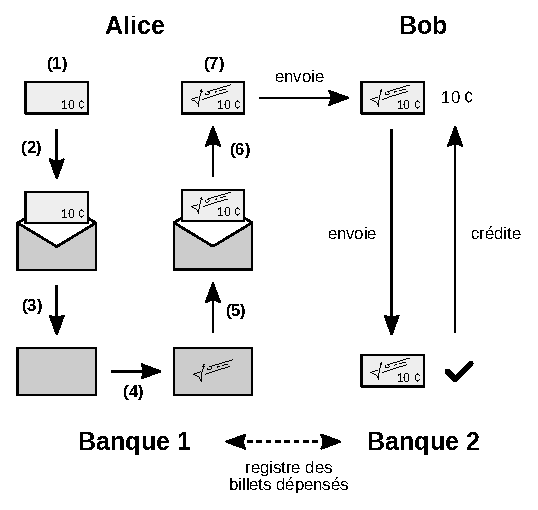
\includegraphics[scale=0.75]{img/chaumian-ecash.eps}
  \caption{Création et remplacement d'un billet chaumien.}
\end{figure}

% Adossement
Les billets numériques peuvent être émis pour eux-mêmes, auquel cas ils forment une monnaie de base. Mais ils peuvent également être adossés à une autre monnaie comme le dollar. Dans ce dernier cas, l'utilisateur peut à tout moment rendre ses billets à sa banque pour récupérer la somme correspondante.

% Confidentialité
La principale conséquence du procédé est qu'aucune banque du système ne peut relier le paiement à l'identité d'Alice. La banque d'Alice sait qu'un billet signé par elle a été dépensé, mais elle ne peut pas savoir de manière absolue qu'il s'agit d'un billet ayant appartenu à Alice. La banque de Bob sait que Bob a reçu le paiement et qu'il provient de la banque d'Alice, mais rien de plus. C'est pour cette raison qu'eCash peut être considéré comme un modèle respectueux de la vie privée.

% Limites
Toutefois, cette confidentialité du système repose sur une supposition forte~: la bienveillance des banques du système. En effet, si une banque voulait obtenir des informations liées à un billet particulier (par exemple sous la pression étatique), elle pourrait les demander à son propriétaire en échange de l'autorisation du transfert. On peut ainsi imaginer un système eCash qui respecte pleinement les normes de surveillance, comme le suggère l'implémentation de Chaum pour une MNBC conceptualisée en 2021\sendnote{David L. Chaum, Christian Grothoff, Thomas Moser, \eng{How to Issue a Central Bank Digital Currency}, mars 2021~: \url{https://www.snb.ch/n/mmr/reference/working_paper_2021_03/source/working_paper_2021_03.n.pdf}.}.

% Enfin, dans la pratique, le système était strictement fermé. La société de David Chaum, DigiCash, possédait le brevet sur le procédé de signature aveugle qui en rendait illégale la reproduction sans son accord. Elle était donc la seule autorité agrémentée pour pouvoir chapeauter un système eCash.

\section*{Magic Money, les CyberBucks et les banques} % Tacky Tokens (26/2/94), CyberBucks (19/10/94), Mark Twain Bank (23/10/95)
\addcontentsline{toc}{section}{Magic Money, les CyberBucks et les banques}

% Mise en application de eCash
Le concept d'eCash a été mis en application au cours des années 90. À l'époque, le Web venait tout juste d'apparaître, le commerce électronique était inexistant et cette idée constituait une formidable opportunité. Cette mise en œuvre a été réalisée d'abord par les cypherpunks par l'intermédiaire du protocole Magic Money, puis par la société de David Chaum, DigiCash, au moyen de jetons d'essai appelés les CyberBucks et d'un déploiement dans le système bancaire classique. % Les cypherpunks ont été enthousiasmé par ces déploiements.

% Magic Money
Le protocole Magic Money a été présenté sur la liste de diffusion des cypherpunks le 4 février 1994 par un développeur anonyme se faisant appeler Pr0duct Cypher et utilisant PGP pour s'identifier. Magic Money permettait de créer sa monnaie en faisant fonctionner un serveur de courrier électronique qui servait de monnaierie eCash\sendnote{«~Magic Money est un système d'argent liquide numérique conçu pour être utilisé par courrier électronique. Le système est en ligne et intraçable. En ligne signifie que chaque transaction implique un échange avec un serveur, pour éviter les doubles dépenses. Intraçable signifie qu'il est impossible pour quiconque de retracer les transactions, de faire correspondre un retrait avec un dépôt, ou de faire correspondre deux pièces de quelque manière que ce soit.~» -- Pr0duct Cypher, \eng{Magic Money Digicash System}, \wtime{04/02/1994 20:44:27 UTC}~: \url{https://cypherpunks.venona.com/date/1994/02/msg00247.html}.}. Magic Money utilisait l'algorithme RSA et la signature aveugle, deux techniques qui étaient brevetées à l'époque, de sorte que son déploiement était \eng{de facto} illégal et devait se confiner à l'expérimentation. Cette annonce a toutefois été accueillie favorablement sur la liste, notamment par Hal Finney\pagenote{«accueillie favorablement sur la liste, notamment par Hal Finney~»~: Hal Finney, \eng{Re: Magic Money Digicash System}, \wtime{04/02/1994 21:58:18 UTC}~: \url{https://cypherpunks.venona.com/date/1994/02/msg00251.html}.}.

% Tacky Tokens et autres jetons fantaisistes
Le premier système basé sur Magic Money a été mis en ligne par Mike Duvos quelques semaines plus tard avec les Tacky Tokens, dont les pièces étaient émises en valeurs de 1, 2, 5, 10, 20, 50 et 100 unités\pagenote{«~Tacky Tokens, dont les pièces étaient émises en valeurs de 1, 2, 5, 10, 20, 50 et 100 unités~»~: Mike Duvos, \eng{Fun With Magic Money}, \wtime{26/02/1994 00:51:40 UTC}~: \url{https://cypherpunks.venona.com/date/1994/02/msg01391.html}.}. Malgré des propositions, aucune transaction réelle n'a été réalisée, ce qui a poussé Tim May à se demander «~pourquoi l'argent liquide numérique [n'était] pas utilisé\sendnote{Timothy C. May, \eng{Why Digital Cash is Not Being Used}, \wtime{03/05/1994 19:48:18 UTC}~: \url{https://cypherpunks.venona.com/date/1994/05/msg00155.html}.}~». D'autres implémentations fantaisistes de Magic Money ont vu le jour par la suite, comme les GhostMarks, les DigiFrancs ou les NexusBucks, mais n'ont pas connu un plus grand succès. L'activité a très rapidement reculé au cours des semaines\pagenote{«~L'activité a très rapidement reculé au cours des semaines~»~: Mike Duvos, \eng{In Search of Genuine DigiCash}, \wtime{16/08/1994 06:06:49 UTC}~: \url{https://cypherpunks.venona.com/date/1994/08/msg00695.html}.}. % «~Je n'ai pas vu de Tacky Token depuis des mois, bien qu'il y avait pas mal d'activité lorsque j'ai rendu mon serveur disponible au début.~»

% DigiCash
Le concept d'eCash a ensuite été mis en pratique par la société DigiCash B.V., fondée par David Chaum en 1990 et basée à Amsterdam aux Pays-Bas, qui avait pour mission de mettre en application les idées du cryptographe\pagenote{«~Le concept d'eCash a ensuite été mis en pratique par la société DigiCash B.V.~»~: La chronologie de DigiCash se retrouve sur le site personnel de David Chaum. -- David L. Chaum, \eng{eCash}~: \url{https://chaum.com/ecash/}.}. Plusieurs cypherpunks ont travaillé pour cette entreprise comme Eric Hughes, Bryce Wilcox (le futur Zooko Wilcox-O'Hearn) et Nick Szabo. Après quelques années de développement, un prototype a été présenté en mai 1994 lors de la première conférence internationale sur le World Wide Web au CERN à Genève\pagenote{«~présenté en mai 1994 lors de la première conférence internationale sur le World Wide Web au CERN~»~: DigiCash, \eng{World's first electronic cash payment over computer networks}, 27 mai 1994~: \url{https://chaum.com/wp-content/uploads/2022/01/05-27-94-World_s-first-electronic-cash-payment-over-computer-networks.pdf}.}.

% CyberBucks (marque déposée par DigiCash)
DigiCash a ensuite réalisé un essai qui a débuté le 19 octobre de cette année, avec l'émission de CyberBucks. Bien que leur nom fasse référence à la monnaie étasunienne («~\eng{a buck}~»), ceux-ci n'étaient pas adossés au dollar et possédaient donc un prix flottant par rapport à ce dernier. Une distribution initiale de 100 CyberBucks par nouvel utilisateur a été effectuée afin d'aider l'amorçage du système. Les cypherpunks se sont appropriés la chose en effectuant des échanges réels~: la récompense pour la résolution d'un problème, la vente de t-shirts, la vente de logiciels, et bien sûr le change avec le dollar\sendnote{Jim Crawley, «~Electronic Cash~», \eng{The Computists' Weekly}, vol. 5, no. 25, 11 juillet 1995~: \url{https://www.nzdl.org/cgi-bin/library?e=d-00000-00---off-0tcc--00-0----0-10-0---0---0direct-10---4-------0-1l--11-ro-50---20-preferences---10-0-1-00-0--4----0-0-11-10-0utfZz-8-00&a=d&cl=CL2.5&d=HASH0199d48acda6ba6861de2d9e.2}.}. Divers commerçants acceptaient les CyberBucks dans le cadre de cette expérience.

% Mark Twain Bank
Mais les CyberBucks ne constituaient qu'une monnaie d'essai, qui a périclité en octobre 1995 lorsque la Mark Twain Bank, une petite banque du Missouri, a lancé sa propre version du protocole en partenariat avec DigiCash. Contrairement à l'essai précédant, l'unité échangée était adossée au dollar étasunien. Bien que l'expérience des CyberBucks ne se soit pas techniquement arrêtée là, leur valeur s'est effondrée à cause de cette nouvelle\sendnote{«~Mark Twain est arrivée sur le marché avec de l'argent liquide numérique \emph{réel}, et les gens ont complètement cessé d'échanger les certificats bêta. Je ne me souviens même pas du dernier prix de règlement, mais il s'agissait de quelques centimes de dollars.~» -- Robert Hettinga, \eng{e\$: Interbank Digital Cash Clearing, Better Living through Walletware, Microintermediation, Net.Currencies and ECM}, 3 juin 1996, archive~: \url{https://web.archive.org/web/19980204144728/http://www.shipwright.com/rants/rant_14.html}.}. % "Last summer, when I got back from my New Orleans trip, I was up in Montana hanging out while my wife was at an educator's conference, and Lucky Green sends me e-mail about having just sold, for cash, some of the demo 'cyberbuck' certificates that Digicash was issuing at the time. I commented about this to cypherpunks, one thing led to another, and the next thing I knew, Rich Lethin had started up a mailing list and set up a protocol for trading these beta-certificates for cash over that list. He named the list ecm. (Send 'info ecm' in the body of a message to majordomo@ai.mit.edu, if you want to see what the fuss was all about.) It was used sporadically up to the time when, you guessed it, Mark Twain came on line with actual digital cash, and people stopped trading beta-certificates altogether. I can't even remember what the last settlement price was, but it was pennies on the dollar. Actually, now that I remember it, there was a period where the beta-certificates were traded for real Mark Twain ecash on someone's web-page and then announced on ecm, but things have pretty much gone moribund on ecm lately. I haven't seen a trade go across in many months."

% Système traditionnel
Par la suite, DigiCash a conclu des partenariats avec différentes banques pour s'inscrire dans le milieu financier traditionnel. Entre 1996 et 1998, six banques situées aux quatres coins du monde ont suivi la Mark Twain Bank~: la Merita Bank en Finlande, la Deutsche Bank en Allemagne, l'Advance Bank en Australie, la Bank Austria en Autriche, la Den norske Bank en Norvège et le Crédit Suisse en Suisse. On lui promettait alors un avenir radieux\sendnote{Antoine Champagne, «~\eng{L'argent liquide numérique (crypto-curency) est né en 1995~: souvenirs}~», \emph{Reflets.info}, 11 janvier 2014~: \url{https://reflets.info/articles/l-argent-liquide-numerique-crypto-curency-est-ne-en-1995-souvenirs}.}.

% Refus de développement
C'était toutefois sans compter sur le caractère de David Chaum, qui était têtu, suspicieux et souhaitait garder le contrôle sur son entreprise\sendnote{«~\eng{Hoe DigiCash alles verknalde}~», \eng{Next! Magazine}, 1\ier{} janvier 1999, archive~: \url{https://web.archive.org/web/19990427142412/https://www.nextmagazine.nl/ecash.htm}. Une traduction (en anglais) est disponible à l'adresse \url{https://cryptome.org/jya/digicrash.htm}.}. Ainsi, ce dernier a refusé des partenariats avec de grands acteurs comme ING et ABN AMRO (deux des trois plus grandes banques néerlandaises à l'époque), Visa, Netscape et Microsoft. Finalement, il a dû, sous pression des actionnaires et des employés, quitter son poste de PDG pour devenir directeur technique et céder sa place à Michael Nash, ancien employé de Visa, en 1997. Le siège social de DigiCash a été déménagé en Californie et l'entreprise est par conséquent devenue une société étasunienne.

% Faillite
Le 17 septembre 1998, la Mark Twain Bank (rachetée par la Mercantile Bancorporation en 1996) a annoncé abandonner eCash, ce qui a provoqué la fin de DigiCash. Le 3 novembre, l'entreprise est entrée en faillite et a été placée sous la protection du chapitre 11 aux États-Unis, de sorte que ses possessions ont été progressivement revendues au fil des années, dont ses brevets en 2002. Avec DigiCash, c'était le concept même d'eCash qui disparaissait de la circulation.

% Raisons
En 1999, Chaum a expliqué les raisons de l'échec de sa société, à savoir le manque d'adoption dû à la difficulté d'utilisation\pagenote{«~le manque d'adoption dû à la difficulté d'utilisation~»~: Julie Pitta, \eng{Requiem for a Bright Idea}, 1\ier{} novembre 1999~: \url{https://www.forbes.com/forbes/1999/1101/6411390a.html}.}. Cette disparition a progressivement laissé les cartes de paiement et PayPal triompher. % David Chaum expliquait~: «~Il était difficile d'amener assez de commerçants à l'accepter de manière à ce qu'assez de consommateurs l'utilisent, ou vice versa. À mesure que le Web grandissait, le niveau moyen de sophistication des utilisateurs baissait. Il était difficile de leur expliquer l'importance de la confidentialité.~»

% Demande pour un argent liquide électronique
La fin de DigiCash a ainsi laissé un vide sur le marché de l'argent liquide numérique. Mais la demande n'a jamais disparu, de sorte qu'on pouvait pressentir qu'il réapparaîtrait d'une façon ou d'une autre. Tel que le prédisait Milton Friedman, prix Nobel d'économie et fondateur de l'École de Chicago, en 1999, au micro de la National Taxpayers Union Foundation~:

\begin{quote}
«~Je pense qu'Internet va devenir l'une des forces majeures qui va réduire le rôle de l'État. La seule chose qui manque, mais qui sera bientôt développée, c'est un argent liquide électronique fiable, une méthode qui permette de transférer des fonds de A à B sur Internet sans que A connaisse B ou que B connaisse A\sendnote{Milton Friedman, \eng{Milton Friedman Full Interview on Anti-Trust and Tech} (vidéo), 1999~: \url{https://www.youtube.com/watch?v=mlwxdyLnMXM}, \wtime{14:32}.}.~»
\end{quote} % "I think that the internet is going to be one of the major forces for reducing the role of government. The one thing that's missing but that will soon be developed, is a reliable e-cash, a method whereby on the internet you can transfer funds from A to B without A knowing B or B knowing A."

\section*{libtech-l~: révolutionner la monnaie}
\addcontentsline{toc}{section}{libtech-l~: révolutionner la monnaie}

Après l'échec d'eCash en octobre 1998, l'idée d'un argent liquide numérique réel a progressivement été délaissée par les cypherpunks, qui se sont contentés pour la plupart des expériences de monnaie privée et des systèmes de paiement existants. Mais ce n'était pas le cas de tous les membres du mouvement. Un petit nombre d'entre eux s'est ainsi regroupé sur une liste de diffusion privée appelée libtech-l où ils ont pu parler de comment la monnaie évoluerait.

% libtech-l
La liste libtech-l, créée en 1994 par Nick Szabo\sendnote{libtech-l@netcom.com -- Timothy C. May, \eng{Re: Regional Lists}, \wtime{28/06/1994 05:48:50 UTC}~: \url{https://cypherpunks.venona.com/date/1994/06/msg01156.html}~; Timothy C. May, \eng{Cyphernomicon}, 2.4.27.}, avait pour but, comme son nom l'indique, d'héberger des discussions sur les techniques libératoires, à même de protéger la liberté individuelle face à l'autorité, dans l'esprit des mouvements extropien et cypherpunk dont les membres étaient par ailleurs des participants. On pouvait y retrouver notamment les interventions des cypherpunks Wei Dai et Hal Finney, ainsi que celles des économistes Larry White et George Selgin. Ces cinq individus formaient le noyau dur de cette liste privée, dont émergeraient plusieurs idées de monnaie numérique.

% Nick Szabo
Nicholas J. Szabo, dit Nick Szabo, était un informaticien américain d'origine hongroise. Extropien, puis cypherpunk, il s'était notamment illustré par son implication dans le combat contre la puce Clipper. En 1994, il avait formalisé la notion de \eng{smart contract}, qu'il avait définie comme «~un protocole de transaction informatisé qui exécute les termes d'un contrat\sendnote{Nick Szabo, \eng{Smart Contracts}, 1994, archive~: \url{https://web.archive.org/web/20011102030833/http://szabo.best.vwh.net:80/smart.contracts.html}.}~», et l'avait approfondie dans les années qui ont suivi\pagenote{«~l'avait approfondie dans les années qui ont suivi~»~: Nick Szabo, «~\eng{Smart Contracts: Building Blocks for Digital Markets}~», \eng{Extropy}, vol. 16, 1\ier{} janvier 1996~: \url{https://github.com/Extropians/Extropy/blob/master/Extropy-16.pdf}~; Nick Szabo, «~\eng{Smart Contracts: Formalizing and Securing Relationships on Public Networks}~», \eng{First Monday}, vol. 2, no. 9, 1\ier{} septembre 1997~: \url{https://firstmonday.org/ojs/index.php/fm/article/view/548/469}.}.  % Il travaille ensuite pour des entreprises technologiques comme JPL, Cuesta Technology ou Arcot Systems. A travaillé pour Agorics

% Centres d'intérêt
Nick Szabo avait une personnalité curieuse et éclectique, de sorte qu'il s'intéressait à une multitude de domaines, tels que l'informatique, l'économie, la politique et la biologie, et écrivait de manière prolifique à leur sujet\sendnote{On peut retrouver les écrits de Nick Szabo sur son ancienne page personnelle szabo.best.vwh.net et sur son blog Unenumerated débuté en 2005. -- Archive de la page personnelle~: \url{https://web.archive.org/web/20160709091851/http://szabo.best.vwh.net/}~; Unenumerated~: \url{https://unenumerated.blogspot.com/}.}. Il avait un intérêt particulier pour le droit, dont il possédait une conception libérale et jusnaturaliste, un intérêt qui le pousserait par la suite à retourner étudier et à obtenir un diplôme dans la discipline en 2006.

% DigiCash et la minimisation de la confiance
Il avait travaillé pendant six mois comme consultant pour DigiCash à Amsterdam vers 1995. Il y avait appris le rôle néfaste (et, finalement, fatal) des tiers de confiance. C'est de cette expérience que provenait son obsession pour la minimisation de la confiance, qu'il s'efforçait à mettre en valeur au sein de ses travaux\sendnote{Nick Szabo, \eng{Trusted Third Parties are Security Holes}, 2001, archive~: \url{https://web.archive.org/web/20020423191203/http://szabo.best.vwh.net/ttps.html}.}.

% Hal Finney
Hal Finney, comme déjà indiqué dans le chapitre précédent, était un informaticien et cryptographe qui vivait dans la région de Los Angeles. Extropien et cypherpunk de la première heure, il travaillait alors pour Phil Zimmermann sur le développement de PGP, officieusement depuis 1992, puis officiellement à partir de 1996. Hal Finney s'était aussi passionné pour les idées de David Chaum dont son fameux eCash\sendnote{«~Lorsque j'ai découvert les travaux de Chaum, j'ai été époustouflé. Le premier article que j'ai trouvé, je crois, était son article dans CACM, qui donnait un aperçu des nombreuses possibilités offertes. J'ai commencé à essayer de retrouver d'autres articles de Chaum. On y trouvait toutes les techniques nécessaires pour faire fonctionner le monde de Vinge, des techniques que Vinge connaissait apparemment déjà, bien avant moi.~» -- Hal Finney, \eng{Why remailers...}, \wtime{16/11/1992 01:30:02 UTC}~: \url{https://cypherpunks.venona.com/date/1992/11/msg00108.html}.}. % "When I found Chaum's stuff, it just blew me away. The first article I found, I think, was his CACM paper which is an overview of many of the things that are possible.  I started trying to track down other papers by Chaum.  Here were all the technologies needed to make Vinge's world work, technologies which Vinge apparently knew about long before I did."

% Wei Dai
Wei Dai était un jeune cryptographe sino-américain vivant à Seattle. Ayant fui la Chine communiste et émigré aux États-Unis avec ses parents à l'âge de 10 ans\pagenote{«~Ayant fui la Chine communiste et émigré aux États-Unis avec sa famille à l'âge de 10 ans~»~: Wei Dai, \eng{A tale from Communist China}, \wtime{18/10/2020 17:37 UTC}~: \url{https://www.lesswrong.com/posts/osYFcQtxnRKB4F4HA/a-tale-from-communist-china}~; Wei Dai, \eng{Re: Tell Your Rationalist Origin Story}, \wtime{15/09/2009 02:53 UTC}~: \url{https://www.lesswrong.com/posts/BHMBBFupzb4s8utts/tell-your-rationalist-origin-story?commentId=ByhZPzBDyYdYs9SRN}.}, il avait réussi à se faire une place dans le monde du travail et avait été rapidement engagé par Microsoft, où il avait participé à l'élaboration de plusieurs brevets\pagenote{«~participé à l'élaboration de plusieurs brevets~»~: Voir les brevets US5724279A et US5724279 assignés à Microsoft. Wei Dai est donc \emph{a priori} son nom civil.}. Il avait découvert le mouvement cypherpunk en 1994 et s'y était joint. Le jeune prodige avait contribué au domaine de la cryptographie notamment avec Crypto++, une bibliothèque de fonctions cryptographiques en C++, et Pipenet, un protocole de communication anonyme\pagenote{«~ Pipenet, un protocole de communication anonyme~»~: Wei Dai, \eng{PipeNet description}, \wtime{20/01/1998 07:53:25 UTC}~: \url{https://cypherpunks.venona.com/date/1998/01/msg00878.html}~; Wei Dai, \eng{PipeNet 1.1}, \wtime{26/11/1998 23:33:49 UTC}~: \url{http://www.weidai.com/pipenet.txt}.}. Il s'était intéressé aux monnaies numériques et aux contrats autonomes à partir de 1995, et avait conceptualisé un modèle de crédit anonyme en 1997\pagenote{«~un modèle de crédit anonyme en 1997~»~: Wei Dai, \eng{anonymous credit}, \wtime{12/04/1997 09:08:04 UTC}~: \url{https://cypherpunks.venona.com/date/1997/04/msg00398.html}.}. En 1998, Wei Dai disait être «~fasciné par la crypto-anarchie de Tim May~», où «~l'État [n'était] pas temporairement anéanti mais définitivement oublié et inutile~» et où «~la violence [était] impossible parce que ses participants ne [pouvaient] pas être reliés à leur vrai nom ou à leur localisation géographique\sendnote{Wei Dai, \eng{b-money}, \wtime{26/11/1998 23:33:49 UTC}, archive~: \url{https://web.archive.org/web/19990219124653/http://www.eskimo.com/~weidai/bmoney.txt}.}~». % issu (comme Szabo) de l'Université de Washington, né après 1976

% Larry White et George Selgin
Lawrence H. White, dit Larry White, et George A. Selgin étaient deux économistes ayant été formés dans des universités prestigieuses. Ils étaient tous les deux inspirés par les idées de l'école autrichienne d'économie, sans pour autant y adhérer pleinement. Ils avaient été marqués par les travaux de Friedrich Hayek, et notamment par son ouvrage \eng{The Denationalization of Money} publié en 1976 qui faisait l'apologie de la concurrence absolue dans le domaine monétaire et bancaire. C'est pourquoi, à partir des années 80, ils s'étaient évertués à promouvoir le système de la banque libre dans lequel des monnaies privées pourraient être librement émises par des sociétés financières, menant à un équilibre de marché.

% Amélioration de la monnaie
Ces individus, présents sur la liste libtech-l, souhaitaient améliorer la monnaie. Ils avaient vu la chute de DigiCash et l'échec d'eCash, et étaient conscients des problèmes liés aux tiers de confiance. C'est ainsi que Wei Dai, Nick Szabo et Hal Finney ont tous les trois développé leur propre concept de monnaie numérique~: Wei Dai a imaginé un concept appelé b-money, Nick Szabo a mis au point un modèle nommé bit gold et Hal Finney a construit le système RPOW.

% Preuve de travail
Leurs projets se fondaient sur la notion de preuve de travail, une notion qui avait été mise en pratique en 1997 par Adam Back avec son algorithme Hashcash, dont le but initial était de fournir un moyen de lutter contre le courrier électronique indésirable\sendnote{Pour une explication technique de la preuve de travail, se référer à la section dédiée dans le chapitre~\ref{ch:confirmation}.}. Le cypherpunk britannique avait pensé à en faire la base d'une monnaie numérique, mais il avait conscience que les preuves de travail ainsi obtenues ne pouvaient pas être transférées d'une manière pleinement distribuée (à cause du problème de la double dépense) et qu'il fallait par conséquent passer par un système de monnaieries à la eCash\sendnote{Adam Back, \eng{Re: Bypassing the Digicash Patents}, \wtime{30/04/1997 09:09:37 UTC}~: \url{https://cypherpunks.venona.com/date/1997/04/msg00822.html}.}. % Adam Back : "hashcash is not directly transferable because to make it distributed, each service provider accepts payment only in cash created for them. You could perhaps setup a digicash style mint (with chaumian ecash) and have the bank only mint cash on receipt of hash collisions addressed to it. However this means you've got to trust the bank not to mint unlimited amounts of money for it's own use.
% So, perhaps you could have multiple banks and let reputation sort them out, if you could arrange the protocols so that it would be apparent if a bank was minting more cash than it had received hash collisions for.  (Say by publishing the collisions, and making it possible to publically verify the quantity of cash in circulation). But if you've got multiple banks then you've got to have an exchange mechanism.  The market could probably take care of this, setting exchange rates based on banks reputations.
% However it would be nicer to have something which required no trust and which had no posssibility of cheating rather than relying on reputation to sort them out."
%
% \begin{quote}
% «~Les exigences cryptographiques d'un tel système seraient les suivantes~: 1) anonyme (préservation de la vie privée, anonymat du bénéficiaire et du payeur)~; 2) distribué (pour qu'il soit difficile de le fermer)~; 3) qu'il ait une certaine rareté intégrée~; 4) qu'il ne nécessite pas de faire confiance à un seul individu~; 5) de préférence hors ligne (difficile à réaliser avec un logiciel pur)~; 6) réutilisable.\sendnote{Adam Back, \eng{Re: Bypassing the Digicash Patents}, \wtime{30/04/1997 09:09:37 UTC}~: \url{https://cypherpunks.venona.com/date/1997/04/msg00822.html}.}~»
% \end{quote} % "The cryptographic requirements for a system such as this would be:
%  1) anonymous (privacy preserving, payee and payer anonymous
%  2) distributed (to make it hard to shut down)
%  3) have some built in scarcity
%  4) require no trust of any one individual
%  5) preferably offline (difficult to do with pure software)
%  6) reusable"

% Idée dans l'air du temps
L'idée d'utiliser ce type de preuve de travail comme base de la devise était répandue. Par exemple, en 1996, Ronald Rivest et Adi Shamir avaient décrit MicroMint, un système de micropaiement centralisé dont les pièces devaient être impossibles à contrefaire grâce à la production de preuves de travail\pagenote{Ronald L. Rivest, Adi Shamir, «~\eng{PayWord and MicroMint: Two Simple Micropayment Schemes}~», in \eng{Security Protocols Workshop}, 1996: pp. 69--87~: \url{https://people.csail.mit.edu/rivest/pubs/RS96a.pdf}. Voir aussi \url{https://people.csail.mit.edu/rivest/pubs/RS96a.slides.pdf}.}. Mais elle manquait d'un bon agencement qui puisse lui donner vie de manière robuste et durable.

\section*{Le concept b-money} % Wei Dai, b-money, 1998
\addcontentsline{toc}{section}{Le concept b-money}

% Description
Le premier concept de monnaie numérique à être sorti de la liste libtech-l était b-money, proposé par Wei Dai. Il s'agissait d'un concept de protocole décentralisé gérant une unité de compte du même nom, la b-money, dont la valeur était censée suivre le cours d'un panier de marchandises.

% Origine
Wei Dai a travaillé sur son idée à partir de 1995\pagenote{«~Wei Dai a travaillé sur son idée à partir de 1995~»~: Wei Dai, \eng{Re: AALWA: Ask any LessWronger anything}, \wtime{16/03/2014 06:14 UTC}~: \url{https://www.lesswrong.com/posts/YdfpDyRpNyypivgdu/aalwa-ask-any-lesswronger-anything?commentId=ZvJDryrskf2Gy6nhG}.}. Comme il l'a expliqué par la suite, sa motivation était de «~rendre possible l'établissement d'une économie en ligne qui soit purement volontaire, une économie qui ne puisse pas être taxée et réglementée par la menace de violence\sendnote{Morgen E. Peck, «~\eng{Bitcoin: The Cryptoanarchists' Answer to Cash}~», \emph{IEEE Spectrum}, 30 mai 2012~: \url{https://spectrum.ieee.org/bitcoin-the-cryptoanarchists-answer-to-cash}.}~». % "My motivation for b-money was to enable online economies that are purely voluntary, ones that couldn't be taxed or regulated through the threat of force."

% Texte de b-money
Le texte descriptif de b-money a été publié le 26 novembre 1998 par Wei Dai sur sa page personnelle\pagenote{«~Le texte descriptif de b-money a été publié le 26 novembre 1998 par Wei Dai sur sa page personnelle~»~: Wei Dai, \eng{b-money}, \wtime{26/11/1998 23:33:49 UTC}, archive~: \url{https://web.archive.org/web/19990219124653/http://www.eskimo.com/~weidai/bmoney.txt}.}. Il en a fortuitement partagé le lien à la liste de diffusion cypherpunk dans un courriel où il décrivait b-money comme «~un nouveau protocole d'échange monétaire et d'exécution des contrats pour les pseudonymes\sendnote{Wei Dai, \eng{PipeNet 1.1 and b-money}, \wtime{26/11/1998 23:33:49 UTC}~: \url{https://cypherpunks.venona.com/date/1998/11/msg00941.html}.}~». % Le texte final (avec l'appendice a été publié en 1999~: voir \url{https://web.archive.org/web/19990502140406/http://www.eskimo.com/~weidai/bmoney.txt} (le texte correspond à http://www.weidai.com/bmoney.txt).

% Deux versions
Le texte était court (un peu plus de 1~000 mots) mais riche conceptuellement. Deux versions du protocole étaient décrites par Wei Dai. L'une était irréalisable mais simple, l'autre était plus complexe mais partait d'hypothèses plus réalistes.

% Version 1, transferts
Dans la première version du protocole, chaque participant faisait partie d'un réseau pair à pair intraçable. Chacun était identifié par un «~pseudonyme numérique~» (c'est-à-dire une clé publique) et chaque message transactionnel était signé par l'expéditeur et chiffré pour le destinataire. Chacun maintenait une base de données séparée qui recensait combien d'unités de b-money possédait chaque pseudonyme.

% Création monétaire
La création monétaire était ouverte à tous les participants et se faisait par preuve de travail en diffusant la solution d'un problème informatique connu et précédemment non résolu. Le nombre d'unités créées dépendait alors du coût de cet effort exprimé par rapport à un panier standard de marchandises, pouvant inclure des métaux précieux par exemple~: lorsque son cours par rapport au panier de marchandises augmentait, les acteurs économiques déployaient plus de puissance de calcul pour abreuver le marché~; à l'inverse lorsque son cours baissait, les acteurs économiques étaient incités à utiliser moins de puissance de calcul, ce qui ralentissait la production de b-money. Il s'agissait donc d'un «~stablecoin~» décentralisé avant l'heure\sendnote{Ce fonctionnement pour garantir la stabilité de la b-money ne manque pas de rappeler le stablecoin géré par Maker DAO sur Ethereum, appelé précisément le dai~! Plus tard, Wei Dai a reproché à Satoshi Nakamoto la politique monétaire fixe de Bitcoin, qui devait entraîner selon lui «~une forte volatilité du prix qui impose un coût élevé pour ses utilisateurs~». -- Wei Dai, \eng{Re: Bitcoins are not digital greenbacks}, \wtime{20/04/2013 07:56 UTC}~: \url{https://www.lesswrong.com/posts/P9jggxRZTMJcjnaPw/bitcoins-are-not-digital-greenbacks?commentId=3XvTroRzb23NpHQDc}.}. % "I would consider Bitcoin to have failed with regard to its monetary policy (because the policy causes high price volatility which imposes a heavy cost on its users, who have to either take undesirable risks or engage in costly hedging in order to use the currency)."

% Contrats
Le système offrait également la possibilité de créer et d'exécuter des contrats directement sur le réseau, grâce à un procédé rudimentaire de dépôt fiduciaire. Dans un contrat, les parties impliquées étaient contraintes de mettre en jeu une caution et de désigner un arbitre qui avait pour rôle d'intervenir en cas de litige. Sans résolution à l'amiable, c'était le réseau qui devait trancher selon les éléments diffusés, la position de l'arbitre étant en théorie privilégiée.

% Version 2 : serveurs, preuve d'enjeu
Dans la seconde version du protocole, le registre de propriété n'était plus conservé par tout le monde, mais uniquement par un sous-ensemble de participants appelés des serveurs. Les participants à une transaction devaient alors vérifier que leur transaction avait bien été traitée en envoyant des requêtes à un échantillon aléatoire de serveurs. Puisqu'il était nécessaire de faire confiance à ceux-ci dans une certaine mesure, un mécanisme économique de preuve d'enjeu était mis en place pour faire en sorte qu'ils restent honnêtes. Chaque serveur devait déposer un montant de b-money sur un compte spécial afin d'être pénalisé en cas de mauvaise conduite, et était en outre contraint de publier régulièrement sa création de monnaie et son registre.

% Limites : absence de BFT, centralisation, contrats rudimentaires, oracles
Le concept de b-money présenté par Wei Dai était donc assez ingénieux pour l'époque. Toutefois, il n'était pas fonctionnel et présentait quelques défauts majeurs. D'abord, la première version du protocole était impossible à mettre en place à grande échelle, notamment parce qu'elle ne résistait pas à la multiplication excessive des identités (attaque Sybil), chacun pouvant ajouter facilement de nouveaux ordinateurs sur le réseau. Ensuite, la seconde version semblait plus réaliste, mais avait pour effet de centraliser le système en un petit nombre de serveurs, le rendant ainsi plus vulnérable aux attaques et à la corruption. Enfin, la stabilité par rapport à un panier de marchandises aurait requis ce qu'on appelle aujourd'hui un système décentralisé d'oracles, ce qui est un problème complexe à résoudre\sendnote{Satoshi avait pensé lui-même au problème de l'oracle. Il écrivait ainsi en février 2009~: «~Il n'y a en effet personne pour agir en tant que banque centrale ou réserve fédérale afin d'ajuster l'offre monétaire au fur et à mesure que le nombre d'utilisateurs augmente. Il aurait fallu qu'un tiers de confiance se charge de déterminer la valeur, car je ne sais pas comment un logiciel pourrait connaître la valeur des choses dans le monde réel. S'il existait un moyen astucieux de le faire, ou si nous voulions faire confiance à quelqu'un pour gérer activement l'offre monétaire afin de l'ancrer à quelque chose, les règles auraient pu être programmées à cet effet.~» -- Satoshi Nakamoto, \eng{Re: Bitcoin open source implementation of P2P currency}, 18 février 2009~: \url{https://p2pfoundation.ning.com/forum/topics/bitcoin-open-source?commentId=2003008:Comment:9562}.}. % "To Sepp's question, indeed there is nobody to act as central bank or federal reserve to adjust the money supply as the population of users grows. That would have required a trusted party to determine the value, because I don't know a way for software to know the real world value of things. If there was some clever way, or if we wanted to trust someone to actively manage the money supply to peg it to something, the rules could have been programmed for that."

% Suite
b-money a attiré l'attention des cypherpunks, et en particulier celle d'Adam Back. Néanmoins, Wei Dai n'a jamais implémenté son modèle, non seulement parce qu'il était dysfonctionnel, mais aussi à cause de sa désillusion à l'égard de la cryptoanarchie. Comme il l'a affirmé en 2014~:

\begin{quote}
«~Je n'ai pris aucune mesure pour coder b-money. Cela a en partie été dû au fait que b-money n'était pas encore un modèle complètement réalisable. Mais si je n'ai pas continué à travailler sur ce modèle, c'est parce que j'étais un peu désenchanté par la cryptoanarchie au moment où j'ai fini d'écrire b-money, et que je ne prévoyais pas qu'un système comme celui-ci, une fois mis en œuvre, pourrait attirer autant d'attention et d'utilisation en dehors d'un petit groupe de cypherpunks inconditionnels\sendnote{Wei Dai, \eng{Re: AALWA: Ask any LessWronger anything}, \wtime{15/03/2014 20:34 UTC}~: \url{https://www.lesswrong.com/posts/YdfpDyRpNyypivgdu/aalwa-ask-any-lesswronger-anything?commentId=XKwphuwm366RegQ3d}.}.~»
\end{quote}

% En réalité, si l'on veut trouver une descendance de la b-money et de la vision de Wei Dai, il faut plutôt chercher du côté d'Ethereum. En effet, nombre de caractéristiques d'Ethereum correspondent à ce qu'aurait pu être b-money~: l'ether n'a pas de quantité limitée bien que son émission soit restreinte, des stablecoins indexés sur des monnaies fiat ou de l'or fleurissent sur la chaîne, le système est basé sur des comptes et il est prévu qu'il passe à une preuve d'enjeu telle que le proposait la deuxième version du protocole b-money. De plus, Ethereum est une sorte de fils spirituel de b-money puisque la plus petite unité du système Ethereum est nommée le wei (tout comme celle de Bitcoin est le satoshi), et que le premier stablecoin décentralisé de la chaîne, géré par Maker DAO, s'appelle le dai !

\section*{Le modèle bit gold} % Nick Szabo, bit gold, 1998, 2005
\addcontentsline{toc}{section}{Le modèle bit gold}

Le deuxième modèle qui a émergé de la liste libtech-l était le système bit gold. Celui-ci était censé gérer la création et les échanges d'une ressource virtuelle appelée le bit gold. Contrairement à l'e-gold qui était garanti par de l'or physique, ou la b-money indexée en théorie sur un panier de marchandises, le bit gold ne devait être adossé à aucun autre bien, mais posséder une rareté infalsifiable intrinsèque, et constituer ainsi un or intégralement numérique. % Nick Szabo avait donc, avant Bitcoin, prophétisé qu'une unité électronique pouvait obtenir de la valeur sans pour autant être liée à une autre marchandise au préalable.

% Origine
C'est au cours de l'année 1998 que Nick Szabo a développé son idée de bit gold, qu'il a décrite initialement sur libtech-l, avant d'héberger une ébauche de livre blanc en 1999 sur son site personnel\sendnote{Nick Szabo, \eng{Bit Gold: Towards Trust-Independent Digital Money}, 2005, archive~: \url{https://web.archive.org/web/20140406003811/http://szabo.best.vwh.net/bitgold.html}.}. Il a présenté bit gold au grand public en décembre 2005 dans un article publié sur son blog Unenumerated\sendnote{Nick Szabo, \eng{Bit gold}, 29 décembre 2005~: \url{https://unenumerated.blogspot.com/2005/12/bit-gold.html}.}. La logique derrière bit gold était de minimiser la confiance dans le but de reproduire autant que possible la cherté de production des métaux précieux dans le cyberespace.

% Preuve de travail
L'élément central du protocole était que la création monétaire se faisait par preuve de travail~: les morceaux de bit gold étaient créés grâce à la puissance de calcul des ordinateurs\sendnote{Le calcul de la preuve de travail dans bit gold ne passait pas par l'inversion partielle d'une fonction de hachage (Hashcash) mais par une \eng{secure benchmark function} qui mesurait la difficulté du problème à résoudre sur une machine précise. Cela devait permettre d'approximer le niveau d'énergie utilisé. -- Voir Nick Szabo, \eng{Intrapolynomial Cryptography}, 1999, archive~: \url{https://web.archive.org/web/20011217091748/http://szabo.best.vwh.net/intrapoly.html}.}. Chaque solution était calculée à partir d'une autre, ce qui conduisait à former une chaîne de preuves de travail. Les acteurs responsables de cette production étaient appelés des «~mineurs~» par Szabo.

% Le processus est le suivant~: Une information de référence publique c0 («~challenge bits~») est créée ; Un «~mineur de bit gold~» génère la preuve de travail s0 à partir de c0 ; Cette preuve de travail est horodatée (t0) de manière sécurisée et distribuée grâce à de multiples services d'horodatage ; Le mineur ajoute cette preuve de travail et son horodatage au registre de propriété, qui est un registre distribué ; La preuve de travail devient la nouvelle information de référence c1, à partir de laquelle est calculée une nouvelle preuve de travail s1, etc.

% Horodatage, enregistrement
La date et l'heure de production de ces preuves de travail étaient certifiées au moyen de serveurs d'horodatage multiples. Cette diversité, bien que peu satisfaisante, permettait de limiter le risque lié à un service particulier.

% Partage du registre
La garantie de la possession et des échanges se faisait par le biais d'un registre public de titres de propriété\pagenote{«~un registre public de titres de propriété~»~: Nick Szabo, \eng{Secure Property Titles with Owner Authority}, 1998, archive~: \url{https://web.archive.org/web/20020202165211/http://szabo.best.vwh.net/securetitle.html}.}. Les utilisateurs étaient identifiés par leur clé publique et signaient les transactions grâce à leur clé privée. Le registre était vérifié et maintenu par un réseau de serveurs appelé «~club de propriété~», serveurs qui se mettaient d'accord par un algorithme de consensus~: le \eng{Byzantine Quorum System} de Malkhi et Reiter\pagenote{«~le \eng{Byzantine Quorum System} de Malkhi et Reiter~»~: Dahlia Malkhi, Michael Reiter, «~\eng{Byzantine quorum systems}~», in \eng{Proceedings of the 29th Annual ACM Symposium on Theory of Computing}, 1997.}. Ainsi, n'importe qui pouvait se référer à ce registre pour connaître le propriétaire d'un morceau de bit gold.

% 3 éléments constitutifs
Il est intéressant de noter que les trois éléments constitutifs de bit gold -- les preuves de travail, leurs horodatages et le registre de propriété -- étaient séparés. En particulier, ils étaient pris en charge par des acteurs différents~: les mineurs, les serveurs d'horodatage et les membres du club de propriété. Plus tard, dans Bitcoin, ces trois éléments seraient combinés en un seul et même concept~: la chaîne de blocs.

% Défauts : non fongibilité, horodatage centralisé, consensus BFT classique
Malgré sa volonté de minimiser la confiance, le système imaginé par Szabo possédait quelques problèmes conceptuels. Tout d'abord, la façon dont étaient produits les morceaux de bit gold faisaient qu'ils n'étaient pas fongibles, c'est-à-dire qu'ils ne pouvaient pas être mélangés entre eux, et devaient donc être évalués sur un marché\pagenote{«~les morceaux de bit gold [...] devaient donc être évalués sur un marché~»~: Nick Szabo, \eng{Bit gold markets}, 10 avril 2008~: \url{https://unenumerated.blogspot.com/2008/04/bit-gold-markets.html}.}, de sorte à pouvoir être utilisés pour servir de base à une réelle unité de compte homogène. Ensuite, bit gold faisait usage de serveurs d'horodatage centralisés, qui formaient des points de défaillance uniques non négligeables. Enfin, le système reposait sur un algorithme de consensus dit «~classique~» qui requérait que les membres du club de propriété soient choisis à l'avance, qu'ils soient connus de tous, et que 66~\% d'entre eux se comportent correctement.

% Mise en œuvre
À l'époque, bit gold était pensé comme un système de règlement permettant de gérer une monnaie de réserve rare, et au-dessus duquel serait construite une économie bancaire libre, si possible utilisant le modèle chaumien. Nick Szabo a longtemps réfléchi à comment mettre en application son idée, redemandant même de l'aide en avril 2008 dans un commentaire sur son blog\sendnote{«~[Bit gold] bénéficierait grandement d'une démonstration, d'un marché expérimental (avec par ex. un tiers de confiance pour se substituer à la sécurité complexe nécessaire au système réel). Quelqu'un veut m'aider à en programmer une~?~» -- Nick Szabo, \eng{Re: Bit gold markets}, 10 avril 2008, archive~: \url{https://web.archive.org/web/20171227190431/http://unenumerated.blogspot.com/2008/04/bit-gold-markets.html?showComment=1207799580000\#c3741843833998921269}.}. Szabo n'a jamais pu mettre en œuvre son concept, contrairement à Hal Finney qui a essayé au moyen de son système RPOW.

\section*{Le système RPOW} % Hal Finney, RPOW, 2004-2005
\addcontentsline{toc}{section}{Le système RPOW}

% Présentation
Hal Finney a repris le concept de Nick Szabo et l'a simplifié pour l'implémenter dans un système inédit~: celui des preuves de travail réutilisables ou \eng{Reusable Proofs of Work}, abrégées en RPOW, qu'il a décrit le 15 août 2004. Ce système se basait sur un serveur transparent qui permettait de rendre transférables les preuves de travail produites par Hashcash. Ainsi, le modèle de sécurité ne venait pas d'un réseau distribué comme dans les cas de b-money et de bit gold\sendnote{Voir Hal Finney, \eng{RPOW Theory}, 15 août 2004, archive~: \url{https://web.archive.org/web/20040815154951/http://rpow.net/theory.html}.}.

% Création monétaire
Dans ce système, les jetons de preuve de travail réutilisable étaient gérés par un serveur qui se chargeait de les signer à l'aide du chiffrement RSA. Ils étaient fabriqués par la production d'une preuve de travail via Hashcash, ou bien à partir d'un jeton de RPOW précédent. Chaque jeton de RPOW se composait d'une valeur (définie comme une puissance de 2) et des données relatives à la signature du serveur. Un utilisateur pouvait par conséquent vérifier lui-même l'intégrité du jeton.

% Serveur central
Le système RPOW reposait sur l'utilisation d'un serveur central qui s'occupait de détruire et de recréer les preuves de travail impliquées dans chaque opération, notamment en vérifiant qu'elles ne faisaient pas l'objet d'une double dépense. Afin d'assurer la divisibilité de l'unité de compte, le système permettait de séparer une RPOW en plusieurs RPOW de valeur moindre et de combiner plusieurs RPOW pour en obtenir une seule.

% Paiement
Lors d'un paiement, l'expéditeur donnait ses jetons de RPOW au destinataire, qui s'empressait de communiquer avec le serveur pour recevoir un ou plusieurs nouveaux jetons, dont la valeur globale était égale à la valeur en entrée. Le fonctionnement des RPOW était ainsi similaire à celui des billets numériques dans eCash~: les jetons de RPOW reposaient sur les informations qu'ils contenaient et pouvaient être transférés de manière confidentielle, mais chaque transaction demandait d'interagir avec le serveur pour garantir l'absence de double dépense.

% Modèle de sécurité
Le modèle de sécurité reposait sur le type de serveur mis en place~: il s'agissait d'un «~serveur transparent\sendnote{Hal Finney, \eng{RPOW Security}, 15 août 2004, archive~: \url{https://web.archive.org/web/20040815154806/http://rpow.net/security.html}.}~» utilisant le cryptoprocesseur IBM 4758 Secure Cryptographic Coprocessor, un cryptoprocesseur de haute sécurité résistant aux falsifications, qui permettait, par un procédé d'authentification conçu par IBM, de vérifier quels programmes étaient exécutés sur la machine. De cette manière, un utilisateur externe pouvait s'assurer à tout instant que le serveur RPOW faisait fonctionner le bon programme, dont le code était par ailleurs disponible publiquement.

% Minimisation de la confiance et confidentialité
Avec son système RPOW, Hal Finney tentait ainsi de réduire la confiance requise à un minimum. Le système était confidentiel dans le sens où l'utilisateur n'avait jamais à s'identifier auprès du serveur et pouvait communiquer avec lui de manière chiffrée. La transparence du serveur permettait, autant que faire se peut, de s'assurer que le système n'était pas corrompu. En particulier, on pouvait rigoureusement supposer que la quantité de jetons de RPOW dépendait d'une production réelle de preuves de travail, propriété qui permettait d'assimiler les jetons de RPOW à de l'or. Il s'agissait, en somme, d'une mise en œuvre partielle du bit gold de Nick Szabo\pagenote{«~Il s'agissait, en somme, d'une mise en œuvre partielle du bit gold de Nick Szabo~»~: À propos du bit gold de Nick Szabo, Hal Finney écrivait~:

\begin{quote}
\footnotesize  «~Le chercheur en sécurité Nick Szabo a inventé le terme bit gold pour désigner un concept similaire de jetons qui représentent intrinsèquement un certain niveau d'effort. Le concept de Nick est plus complexe que le système simple des RPOW, mais son idée s'applique~: à certains égards, un jeton de RPOW peut être considéré comme ayant les propriétés d'une substance rare comme l'or. Miner et frapper des pièces d'or demande un effort et une dépense, ce qui les rend intrinsèquement rares. Les pièces d'or peuvent alors être transmises d'une personne à une autre, et chaque bénéficiaire peut vérifier l'authenticité de la frappe monétaire.

De la même manière, la création de jetons de RPOW demande un certain degré d'effort et de dépense. Ils débutent tous avec une collision hashcash qui, au plus haut degré, prendra des heures voire des jours de calcul pour être créée. Les jetons de RPOW peuvent être validés et vérifiés à la réception en étant échangés contre un nouveau jeton de RPOW sur un serveur RPOW. Cela leur permet d'être transmis d'une personne à une autre tout comme des pièces.

Plus important encore, le système RPOW est conçu dans un but primordial~: empêcher quiconque, y compris le propriétaire du serveur RPOW et le développeur du logiciel RPOW, de violer les règles du système et de falsifier des jetons de RPOW. Sans cette garantie contre la falsification, les jetons de RPOW ne représenteraient pas de manière crédible le travail effectué pour les créer. Des jetons falsifiables ressembleraient davantage à du papier-monnaie qu'à du bit gold. Mon objectif avec ce projet était de donner vie à une concrétisation simple qui démontre la puissance du concept de bit gold. Pour ce faire, une résistance à la falsification est nécessaire, et c'est cet objectif qui a dominé tous les aspects de la conception.~»
\end{quote}
Hal Finney, \eng{RPOW Theory}, 15 août 2004~: \url{http://rpow.net/theory.html}~; archive~: \url{https://web.archive.org/web/20040815154951/http://rpow.net/theory.html}.}. % "Security researcher Nick Szabo has coined the term bit gold to refer to a similar concept of tokens which inherently represent a certain level of effort. Nick's concept is more complex than the simple RPOW system, but his insight applies: in some ways, an RPOW token can be thought of as having the properties of a rare substance like gold. It takes effort and expense to mine and mint gold coins, making them inherently scarce. Gold coins can then be passed from person to person, and each recipient can verify the authenticity of the coinage.
%
% In a similar way, RPOW tokens take a certain level of effort and expense to be created. They all start with a hashcash collision which, at the higher levels, will take hours or even days of computing time to create. RPOW tokens can be validated and verified upon receipt by exchanging them at the RPOW server for a new RPOW token. This allows them to be passed from person to person much like coins.
%
% Most importantly, the RPOW system is architected with one overriding goal: to make it impossible for anyone, even the owner of the RPOW server, even the developer of the RPOW software, to be able to violate the system's rules and forge RPOW tokens. Without such a guarantee against forgeability, RPOW tokens would not credibly represent the work that was done to create them. Forgeable tokens would be more like paper money than bit gold. My goal in this project was to bring to life a simple realization which demonstrates the power of the bit gold concept. This requires resistance to forgeability, and this goal has dominated every part of the design."

% Réalisation
Le système a été lancé en production le même jour que sa description, le 15 août 2004. Hal Finney l'a annoncé sur la liste des cypherpunks\pagenote{«~Hal Finney l'a annoncé sur la liste des cypherpunks~»~: Hal Finney, \eng{RPOW - Reusable Proofs of Work}, \wtime{15/08/2004 17:43:09 UTC}~: \url{https://lists.cpunks.org/pipermail/cypherpunks-legacy/2004-August/134945.html}.} et l'annonce a été retransmise sur la liste de Metzdowd.com par Robert Hettinga\pagenote{«~l'annonce a été retransmise sur la liste de Metzdowd.com par Robert Hettinga~»~: Robert Hettinga, \eng{FW: RPOW - Reusable Proofs of Work}, \wtime{15/08/2004 18:36:51 UTC}~: \url{https://www.metzdowd.com/pipermail/cryptography/2004-August/007362.html}.}. Le système a été mis à jour plusieurs fois pour améliorer son fonctionnement et est resté opérationnel pendant des mois.

% Présentation et avenir
Hal Finney a présenté son système à la CodeCon 2005 organisée à San Francisco. Il y a fait part des usages qu'il envisageait pour RPOW à savoir le transfert de la valeur, la régulation du courrier indésirable (dans la droite lignée de Hashcash), le commerce dans les jeux vidéos, le jeu d'argent en ligne comme le poker, et l'anti-parasitisme sur les protocoles de partage de fichiers comme BitTorrent\sendnote{Hal Finney, \eng{Reusable Proofs of Work}, 1\ier{} février 2005, archive~: \url{https://web.archive.org/web/20050204193327/http://rpow.net/slides/slide001.html}.}. Fidèle à son optimisme, Hal Finney envisageait un avenir prometteur pour RPOW et comptait notamment multiplier le nombre de serveurs autour du monde, une fois que son déploiement initial serait réalisé\pagenote{«~comptait notamment multiplier le nombre de serveurs autour du monde~»~: Hal Finney, \eng{World of RPOW}, 15 août 2004~: \url{http://rpow.net/world.html}~; archive~: \url{https://web.archive.org/web/20040816004128/http://rpow.net/world.html}.}.

% Limites
Toutefois, RPOW présentait des défauts intrinsèques qui peuvent expliquer pourquoi il n'a pas rencontré le succès escompté. L'inconvénient majeur était son modèle de sécurité qui démontrait une certaine faiblesse~: le ou les serveurs devaient être connus et pouvaient être arrêtés facilement, de sorte qu'ils constituaient des points de défaillance unique. De plus, un autre inconvénient venait de sa politique monétaire qui, bien que théoriquement viable, n'était pas spécialement attractive en raison de la hausse exponentielle des performances informatiques.

% Utilisation
De ce fait, l'utilisation réelle de RPOW a été anecdotique. Le système était loin d'être parfait et ne pouvait pas, de toute évidence, devenir un système monétaire solide. Toutefois, il a eu le mérite de constituer une preuve de concept expérimentale, quatre ans avant Bitcoin. % Le site rpow.net a été abandonné en 2010.

\section*{Le projet Ripple} % Ryan Fugger, Ripple classique, 2004-2012
\addcontentsline{toc}{section}{Le projet Ripple}

% Description
Les cypherpunks n'étaient pas les seuls à essayer de construire des systèmes distribués qui puissent servir à l'échange monétaire. C'était le cas du développeur canadien Ryan Fugger, qui en 2004 a conçu un protocole de crédit distribué du nom de Ripple. Ce protocole s'inspirait du concept du système d'échange local (SEL) imaginé par Michael Linton dans les années 1980. Fugger lui-même avait participé à un tel système à Vancouver avant de concevoir Ripple\pagenote{«~Fugger lui-même avait participé à un tel système à Vancouver~»~: Bailey Reutzel, \eng{Disruptor Chris Larsen Returns with a Bitcoin-Like Payment System}, 7 décembre 2012~: \url{https://www.americanbanker.com/news/disruptor-chris-larsen-returns-with-a-bitcoin-like-payment-system}~; archive~: \url{https://web.archive.org/web/20140323151243/http://www.paymentssource.com/news/disruptor-chris-larsen-returns-with-bitcoin-like-payments-system-3012580-1.html?zkPrintable=1\&nopagination=1}.}. Son invention était ainsi un pur produit du localisme monétaire. % Michael Linton : écossais vivant à Vancouver

% Ripple
Ryan Fugger a publié le livre blanc de Ripple en 2004\sendnote{Ryan Fugger, \eng{Money as IOUs in Social Trust Networks \& A Proposal for a Decentralized Currency Network Protocol}, version 2, 18 avril 2004, archive~: \url{https://web.archive.org/web/20060221162102/http://ripple.sourceforge.net/decentralizedcurrency.pdf}.}. Le concept se fondait sur l'idée que la monnaie était essentiellement constituée de reconnaissances de dette (\eng{IOUs}), c'est-à-dire de crédit.

% Réseau de confiance
Le système Ripple s'établissait sur un réseau pair à pair dont les liens étaient des relations de crédit entre des personnes. Chaque relation était composée de deux paramètres~: la dette existante, qui indiquait combien une partie devait à l'autre, et la dette potentielle, qui prenait en compte la propension à prêter et à emprunter des deux parties. Ripple constituait ainsi un système où tous les participants étaient des banquiers. Concernant la monnaie de base, le protocole pouvait gérer de multiples unités de compte (du dollar, de l'euro ou même des heures de travail), mais celles-ci devaient être converties pour être transférées dans une autre devise.

% Paiement
Dans Ripple, les paiements se faisaient par le routage d'une série d'emprunts. En supposant des relations de confiance entre Alice et Bob, Bob et Carole, et Carole et David, Alice réalisait un paiement de 10~\$ vers David en prêtant 10~\$ à Bob, et en demandant à Bob de faire de même auprès de Carole, puis à Carole de faire de même auprès de David. Le compte de David était alors crédité de 10~\$ issus de la création monétaire d'Alice. Ce fonctionnement par propagation du crédit au sein d'un réseau de confiance explique le nom du projet, le mot \eng{ripple} signifiant ondulation en anglais.

% Compensation et règlement
La compensation se faisait par la découverte de cycles de crédit dans le réseau. Si Bob devait 5~\$ à Alice, Carole 5~\$ à Bob et Alice 5~\$ à Carole, alors leurs dettes mutuelles disparaissaient, ce qui permettait à tous les acteurs d'avoir une capacité d'emprunt plus grande pour recevoir de futurs paiements. Une dette pouvait également être éteinte par son règlement entre les deux parties dans l'unité de compte indiquée.

% Preuve de concept (Ripplepay et Google Group.
En 2006, dans l'idée de faire progresser son projet, Ryan Fugger a mis en ligne une preuve de concept appelée Ripplepay\pagenote{«~une preuve de concept appelée Ripplepay~»~: \url{https://web.archive.org/web/20070702210719/http://ripplepay.com/}.}. Celle-ci était basée sur un serveur central (\longstring{ripplepay.com}) et permettait aux utilisateurs de se connecter avec une simple adresse de courrier électronique. Ryan Fugger a également créé un Google Group en janvier 2007\pagenote{«~Ryan Fugger a également créé un Google Group en janvier 2007~»~: Ryan Fugger, \eng{Welcome...}, \wtime{14/01/2007 23:47:26 UTC}~: \url{https://groups.google.com/g/rippleusers/c/oRDaKz-qPjQ/m/zHV3hMPwMg0J}.}.

% Limites
Malgré l'enthousiasme de sa communauté et quelques milliers d'utilisateurs, Ripple possédait des défauts inhérents à son fonctionnement distribué. En particulier, il souffrait du «~problème de l'engagement décentralisé\sendnote{fiatjaf, \eng{Ripple and the problem of the decentralized commit}, \wtime{17/10/2020 13:56 UTC}~: \url{https://fiatjaf.com/3cb7c325.html}.}~»~: durant un paiement, les participants ne pouvaient pas s'engager d'une façon sûre pour assurer la chaîne de prêts\sendnote{Ce problème a été résolu d'une certaine manière par le réseau Lightning qui possède la même structure que Ripple, à l'exception que l'unité échangée n'est pas du crédit à proprement parler. -- Voir fiatjaf, \eng{The Lightning Network solves the problem of the decentralized commit}, \wtime{19/10/2020 19:09 UTC}~: \url{https://fiatjaf.com/e3624832.html}.}.

% Vers XRP
Voyant que son implémentation n'allait nulle part, Ryan Fugger a laissé les rênes de son projet entre les mains des dirigeants de l'entreprise OpenCoin Inc., Chris Larsen et Jed McCaleb, en novembre 2012, qui l'avaient approché quelques mois plus tôt\pagenote{«~Ryan Fugger a laissé les rênes de son projet entre les mains des dirigeants de l'entreprise OpenCoin Inc., Chris Larsen et Jed McCaleb, en novembre 2012~»~: Ryan Fugger, \eng{Ripple.com and taking the project to the next level}, \wtime{28/11/2012 21:21:12 UTC}~: \url{https://groups.google.com/g/rippleusers/c/IVin3Qwrp7k/m/urzaH_VrQcQJ}.}. Ces derniers voulaient combiner son idée avec un nouvel algorithme de consensus, développé par Jed, David Schwartz et Arthur Britto. Le résultat a été sensiblement différent du concept initial, faisant intervenir une unité de compte native, le XRP, et étant bien plus centralisé et contrôlé que ce qu'on attendrait d'un protocole de crédit universel. La société OpenCoin a été rebaptisée Ripple Labs en 2013. Ryan Fugger a finalement modifié le nom de sa preuve de concept en Rumplepay en 2020 pour éviter la confusion\pagenote{«~Ryan Fugger a finalement modifié le nom de sa preuve de concept en Rumplepay en 2020 pour éviter la confusion~»~: Ryan Fugger, \eng{New Name}, 26 août 2020~: \url{https://rumplepay.com/}.}.

\section*{Vers Bitcoin}
\addcontentsline{toc}{section}{Vers Bitcoin}

% Vers Bitcoin
Tous ces concepts de monnaie numérique ont, directement ou indirectement, mené à Bitcoin, soit parce que Satoshi Nakamoto avait connaissance de ces projets, soit parce qu'il partageait les mêmes références que leurs inventeurs. Bitcoin constituait en effet l'aboutissement de ces tentatives de construire une forme de monnaie numérique native du cyberespace.

% Satoshi Nakamoto et eCash
Tout d'abord, Satoshi Nakamoto était pleinement familier de l'eCash de David Chaum et avait de toute évidence lu les échanges des cypherpunks à son sujet. Dans le livre blanc de Bitcoin, il y faisait clairement référence au moment d'aborder le problème de la double dépense tout en utilisant le terme \eng{mint} (traduit ici par monnaierie), qui était un vocable courant parmi les cypherpunks pour désigner les banques chaumiennes~:

\begin{quote}
«~Une solution courante consiste à introduire une autorité centrale de confiance, ou monnaierie, qui vérifie chaque transaction pour s'assurer qu'il n'y a pas de double dépense\sendnote{Satoshi Nakamoto, \eng{Bitcoin: A Peer-to-Peer Electronic Cash System}, 31 octobre 2008.}.~»
\end{quote}

De plus, Satoshi Nakamoto a explicitement reconnu la faiblesse de eCash dans ses interventions publiques et privées. Ainsi, dans un courriel adressé à la liste de diffusion p2p-research en février 2009, il réagissait à la comparaison entre Bitcoin et eCash par Martien van Steenbergen en disant~:

\begin{quote}
«~Bien sûr, la plus grande différence est l'absence de serveur central. C'était le talon d'Achille des systèmes chaumiens~: lorsque l'entreprise centrale fermait ses portes, la monnaie disparaissait\sendnote{Satoshi Nakamoto, \eng{[p2p-research] Re: Bitcoin open source implementation of P2P currency}, \wtime{12/02/2009 19:01:24 UTC}~: \url{https://diyhpl.us/~bryan/irc/bitcoin-satoshi/p2presearch-again/p2pfoundation.net/backups/p2p_research-archives/2009-February.txt.gz}.}.~»
\end{quote} % "Of course, the biggest difference is the lack of a central server.  That was the Achilles heel of Chaumian systems; when the central company shut down, so did the currency."

En privé, il écrivait aussi à Dustin Trammell en 2009~:

\begin{quote}
«~Je pense qu'il y avait beaucoup plus de gens qui étaient intéressés [par la monnaie électronique] dans les années 90, mais après plus d'une décennie d'échecs de systèmes basés sur des tiers de confiance (Digicash,~etc.), ils considèrent qu'il s'agit d'une cause perdue. J'espère qu'ils sauront distinguer que c'est la première fois, à ma connaissance, que nous essayons un système qui n'est pas fondé sur la confiance\sendnote{Satoshi Nakamoto, \eng{Re: Bitcoin v0.1 released}, \wtime{13/01/2009 07:55:20 UTC}~: \url{http://web.archive.org/web/20131204164149/http://www.dustintrammell.com/files/Satoshi_Nakamoto.zip}. -- Il a fait une remarque similaire sur le forum de la Fondation P2P. Voir Satoshi Nakamoto, \eng{Re: Bitcoin open source implementation of P2P currency}, 15 février 2009~: \url{https://p2pfoundation.ning.com/forum/topics/bitcoin-open-source?commentId=2003008:Comment:9493}.}.~»
\end{quote}

La dernière référence au modèle de Chaum était la première version du livre blanc datant du mois d'août 2008 qui s'intitulait de façon limpide «~\eng{Electronic Cash Without a Trusted Third Party}~» («~Un argent liquide électronique sans tiers de confiance~» en français) et dont le nom du fichier était \longstring{ecash.pdf}\sendnote{Gwern Branwen, \emph{Wei Dai/Satoshi Nakamoto 2009 Bitcoin emails}, 17 mars 2014~: \url{https://gwern.net/doc/bitcoin/2008-nakamoto}.}.

% Ignorance de b-money, bit gold et RPOW
Satoshi Nakamoto s'était donc clairement intéressé à eCash avant de concevoir Bitcoin. Toutefois, ce n'était pas le cas des concepts de b-money, bit gold et RPOW, dont il n'avait vraisemblablement pas connaissance en 2007. Ces systèmes ont cependant joué un rôle indirect dans l'histoire de Bitcoin.

% b-money
Comme raconté dans le chapitre~\ref{ch:mythe}, dans sa préparation à la publication de son concept en août 2008, Satoshi est rentré en contact avec Adam Back, qui l'a renvoyé vers Wei Dai, car le britannique avait remarqué les similitudes de Bitcoin avec b-money. C'est à ce moment-là que Satoshi a ajouté la référence à b-money au livre blanc.

% bit gold
Satoshi a appris l'existence du modèle bit gold imaginé par Szabo plus tard, probablement grâce à la première intervention de Hal Finney sur la liste de diffusion le 7 novembre 2008. Ce dernier a instantanément noté la similarité entre Bitcoin et le système de Szabo~:

\begin{quote}
«~Je crois aussi qu'il y a une valeur potentielle dans une forme de jeton infalsifiable dont le taux de production est prévisible et ne peut pas être influencé par des acteurs corrompus. Un tel jeton serait plus comparable à l'or qu'aux monnaies fiat. Nick Szabo a décrit il y a plusieurs années un concept qu'il appelait “bit gold”, et il pourrait s'agir d'une mise en œuvre de cette idée\sendnote{Hal Finney, \eng{Bitcoin P2P e-cash paper}, \wtime{07/11/2008 23:40:12 UTC}~: \url{https://www.metzdowd.com/pipermail/cryptography/2008-November/014827.html}.}.~»
\end{quote}

La référence à bit gold a fini par être ajoutée sur la page web de Bitcoin.org au début de l'année 2009, aux côtés du lien vers le texte descriptif de b-money\pagenote{«~La référence à bit gold a fini par être ajoutée sur la page web de Bitcoin.org au début de l'année 2009~»~: \url{https://web.archive.org/web/20090303195936/http://bitcoin.org/}.}.

% Reconnaissance de b-money et bit gold
Satoshi Nakamoto a reconnu \emph{a posteriori} la ressemblance de ces deux concepts avec son propre modèle. Le 20 juillet 2010, au sein d'une discussion sur le forum parlant de la possible suppression de l'article concernant Bitcoin par Wikipédia, il écrivait pour montrer le sérieux du projet~:

\begin{quote}
«~Bitcoin est une implémentation de la b-money proposée par Wei Dai sur la liste de diffusion des Cypherpunks en 1998 et du Bitgold proposé par Nick Szabo\sendnote{Satoshi Nakamoto, \eng{Re: They want to delete the Wikipedia article}, \wtime{20/07/2010 18:38:28 UTC}~: \url{https://bitcointalk.org/index.php?topic=342.msg4508\#msg4508}.}.~»
\end{quote}

Cette phrase, censée démontrer l'inscription de Bitcoin dans l'histoire de la monnaie numérique, est restée gravée dans les esprits, à tel point que la b-money et le bit gold sont régulièrement cités comme des précurseurs de la cryptomonnaie.

% RPOW
En revanche, Satoshi Nakamoto n'a jamais indiqué à une seule occasion qu'il connaissait le système RPOW de Hal Finney\sendnote{Satoshi Nakamoto a en réalité fait mention de RPOW à Martti Malmi dans un courriel privé qui a été rendu public en février 2024. Voir Satoshi Nakamoto, \eng{Re: Bitcoin}, \wtime{21/07/2009 03:14:43 UTC} : \url{https://mmalmi.github.io/satoshi/\#email-24}. (Note de janvier 2025.)}. Celui-ci n'était après tout qu'un modèle eCash basé sur la preuve de travail, dont le serveur central avait la particularité d'être transparent aux yeux des utilisateurs. Néanmoins, Hal Finney a joué un rôle majeur dans les débuts de Bitcoin et a évoqué son système en 2013 sur Bitcointalk\sendnote{«~Je m'intéressais depuis longtemps aux systèmes de paiement cryptographiques. De plus, j'avais eu la chance de rencontrer et de correspondre longuement avec Wei Dai et Nick Szabo, qui sont généralement reconnus pour avoir créé des idées qui allaient se concrétiser avec Bitcoin. J'avais tenté de créer ma propre monnaie basée sur la preuve de travail, appelée RPOW. J'ai donc trouvé Bitcoin fascinant.~» -- Hal Finney, \emph{Bitcoin and me}, \wtime{19/03/2013 20:40:02 UTC}~: \url{https://bitcointalk.org/index.php?topic=155054.msg1643833\#msg1643833}.}, de sorte que RPOW est aujourd'hui lui aussi considéré comme un prédécesseur de la découverte de Satoshi. % "I was more positive. I had long been interested in cryptographic payment schemes. Plus I was lucky enough to meet and extensively correspond with both Wei Dai and Nick Szabo, generally acknowledged to have created ideas that would be realized with Bitcoin. I had made an attempt to create my own proof of work based currency, called RPOW. So I found Bitcoin facinating."

% Réelle identité, explicaiton de la similitude
La proximité des idées de ces trois hommes avec Bitcoin est étonnante de prime abord, si bien que beaucoup ont spéculé que Satoshi Nakamoto était l'un ou plusieurs d'entre eux. Ces hommes, qui ont avoué avoir découvert l'existence de Bitcoin assez rapidement (Wei Dai lorsque Satoshi l'a contacté en août 2008, Hal Finney lors de la publication du livre blanc, Nick Szabo courant 2009\pagenote{«~Nick Szabo courant 2009~»~: Nick Szabo, \eng{Liar-resistant government}, \wtime{07/05/2009 23:13 UTC}~: \url{https://unenumerated.blogspot.com/2009/05/liar-resistant-government.html}.}), avaient le profil pour avoir imaginé le concept, malgré quelques éléments contradictoires. Cependant, ils ont tous les trois démenti la chose\pagenote{«~ils ont tous les trois démenti la chose~»~: Wei Dai~: «~Ce que je comprends c'est que le créateur de Bitcoin, qui se fait appeler Satoshi Nakamoto, n'a même pas lu mon article avant de réinventer l'idée lui-même. Il l'a appris par la suite et m'a crédité dans son papier. Donc ma connexion avec le projet est assez limitée.~» -- Wei Dai, \eng{Re: Making money with Bitcoin?}, \wtime{25/02/2011 15:27 UTC}~: \url{https://www.lesswrong.com/posts/ijr8rsyvJci2edxot/making-money-with-bitcoin?commentId=hbEu9ue9eymNzaF2J}.

Nick Szabo~: «~Comme je l'ai déclaré à plusieurs reprises auparavant, toute cette spéculation est flatteuse, mais incorrecte -- je ne suis pas Satoshi.~» -- Nathaniel Popper, \eng{Decoding the Enigma of Satoshi Nakamoto and the Birth of Bitcoin}, 15 mai 2015.

Hal Finney~: «~Aujourd'hui, la véritable identité de Satoshi est devenue un mystère. Mais à l'époque, je pensais avoir affaire à un jeune homme d'origine japonaise, très intelligent et sincère.~» -- Hal Finney, \emph{Bitcoin and me}, \wtime{19/03/2013 20:40:02 UTC}~: \url{https://bitcointalk.org/index.php?topic=155054.msg1643833\#msg1643833}.}. % Dai: "my understanding is that the creator of Bitcoin, who goes by the name Satoshi Nakamoto, didn't even read my article before reinventing the idea himself. He learned about it afterward and credited me in his paper. So my connection with the project is quite limited."
% Szabo: "As I've stated many times before, all this speculation is flattering, but wrong — I am not Satoshi."
% "I categorically deny any familiarity with Dorian Nakamoto"

% Wei Dai s'est mis à miner lorsqu'il a redécouvert Bitcoin en 2011\sendnote{Wei Dai, \eng{Re: Making money with Bitcoin?}, \wtime{25/02/2011 15:27 UTC}~: \url{https://www.lesswrong.com/posts/ijr8rsyvJci2edxot/making-money-with-bitcoin?commentId=hbEu9ue9eymNzaF2J}.}.

% Ripple
Le dernier projet de monnaie numérique qui a marqué l'histoire de Bitcoin est le projet Ripple de Ryan Fugger. Même si celui-ci ne ressemblait pas vraiment à Bitcoin, il a néanmoins eu son influence sur le développement de ce dernier. Satoshi Nakamoto connaissait en effet Ripple. En février 2009, sur la liste de diffusion de la Fondation P2P, il répondait à Martien van Steenbergen qui y faisait référence\pagenote{«~il répondait à Martien van Steenbergen qui y faisait référence~»~: Martien van Steenbergen faisait aussi référence à d'autres projets issus de la communauté P2P~: Pekunio et Wizard Rabbit Treasurer. -- Martien van Steenbergen, \eng{[p2p-research] Re: Bitcoin open source implementation of P2P currency}, \wtime{12/02/2009 20:01:03 UTC}~: \url{https://diyhpl.us/~bryan/irc/bitcoin-satoshi/p2presearch-again/p2pfoundation.net/backups/p2p_research-archives/2009-February.txt.gz}.}~:

\begin{quote}
«~En ce qui concerne les systèmes de confiance, Ripple est unique en ce qu'il répartit la confiance plutôt que de la concentrer\sendnote{Satoshi Nakamoto, \eng{[p2p-research] Re: Bitcoin open source implementation of P2P currency}, \wtime{13/02/2009 02:31:20}~: \url{https://diyhpl.us/~bryan/irc/bitcoin-satoshi/p2presearch-again/p2pfoundation.net/backups/p2p_research-archives/2009-February.txt.gz}.}.~»
\end{quote}

Le deuxième lien entre Ripple et Bitcoin est l'implication du développeur Mike Hearn. Ce dernier s'était intéressé au Ripple de Ryan Fugger dès ses débuts et, en 2007, il avait été l'une des premières personnes à intervenir sur le Google Group nouvellement créé\pagenote{«~il avait été l'une des premières personnes à intervenir sur le Google Group nouvellement créé~»~: Mike Hearn, \eng{Hello from a Ripple fan}, \wtime{06/05/2007 12:20:53 UTC}~: \url{https://groups.google.com/g/rippleusers/c/i8OyR5yLC0Q/m/SyztfhBGYJEJ}.}. En découvrant Bitcoin en avril 2009, Hearn n'a ainsi pas pu s'empêcher de demander à Satoshi Nakamoto ce qu'il pensait de ce modèle alternatif, et ce dernier lui a alors répondu que Ripple était «~intéressant~» dans la mesure où c'était «~le seul autre système qui [faisait] quelque chose de la confiance en dehors de la concentrer au sein d'un serveur central\sendnote{Satoshi Nakamoto, \eng{Re: Questions about BitCoin}, \wtime{12/04/2009 20:44 UTC}~: \url{https://plan99.net/\~mike/satoshi-emails/thread1.html}.}~».

% Différence, avis de Fugger
Mais Ripple différait sensiblement de Bitcoin, en particulier par le fait qu'il constituait, à proprement parler, un système de crédit distribué et non pas une monnaie de base décentralisée. C'est ce qui a éloigné Ryan Fugger, qui ne voyait pas «~pourquoi un bitcoin aurait une quelconque valeur, puisqu'il n'y avait apparemment rien pour le garantir~», mais qui s'est finalement rendu à l'évidence que le modèle de Satoshi Nakamoto était «~une excellente idée\sendnote{Ryan Fugger, \eng{Re: Is the cryptocurrency Bitcoin a good idea?}, \wtime{17/05/2011 07:44:33 UTC}~: \url{https://www.quora.com/Is-the-cryptocurrency-Bitcoin-a-good-idea/answer/Ryan-Fugger}.}~».

% Dernière pierre
Bitcoin ajoutait donc la dernière pierre à l'édifice de l'argent liquide électronique. Il apportait enfin une technique permettant de construire une monnaie numérique réellement solide et durable. Le 26 janvier 2009, Zooko Wilcox-O'Hearn témoignait de cette volonté dans un article de blog, qui serait relayé quelques semaines plus tard sur Bitcoin.org. En voici le texte intégral~:

\begin{quote}
«~Depuis quelque temps, je réfléchis à la manière dont des services de jeux comme \emph{World of Warcraft} et \emph{Second Life} (qui prétend ne pas être un jeu) ont réussi là où nous, à DigiCash, avons échoué~: développer un argent liquide numérique programmable, pratique et largement utilisé. Le problème est que toute nouvelle monnaie de ce type est contrôlée de manière centralisée par une seule entité, ce qui limite le champ d'action des gens qui dépendent d'elle et la valeur qu'ils sont prêts à risquer dessus. Certaines pistes sont évoquées pour faciliter le change entre les monnaies, mais cette approche ne résoudra pas le problème. \emph{Une pléthore de services centralisés concurrents n'est pas la même chose qu'un service décentralisé.} Même s'il était bon marché et commode d'échanger des LindenBucks contre de l'or de WoW, on ne ferait que revenir à l'équivalent des monnaies des États-nations modernes~: des monnaies essentiellement centralisées (en raison de \emph{l'effet de réseau}), lourdement taxées\,/\,réglementées\,/\,manipulées, et sujettes à des effondrements désastreux. Ce que je veux, c'est une monnaie que tout le monde puisse utiliser de manière pratique et peu coûteuse, mais que \emph{personne} n'ait le pouvoir de manipuler. Je veux que personne n'ait le pouvoir de gonfler ou de dégonfler la masse monétaire~; que personne n'ait le pouvoir de surveiller, de taxer ou d'empêcher les transactions. Un véritable équivalent numérique de l'or, dans les périodes et les lieux où l'or était la monnaie universelle. Voyez l'idée de BitGold de Nick Szabo et l'idée de b-money de Wei Dai, ainsi que la récente tentative de mettre en œuvre un système de ce genre~: le BitCoin de Satoshi Nakamoto\sendnote{Zooko Wilcox-O'Hearn, \eng{Decentralized Money}, 26 janvier 2009, archive~: \url{https://web.archive.org/web/20090303195936/http://testgrid.allmydata.org:3567/uri/URI:DIR2-RO:j74uhg25nwdpjpacl6rkat2yhm:kav7ijeft5h7r7rxdp5bgtlt3viv32yabqajkrdykozia5544jqa/wiki.html\#\%5B\%5BDecentralized\%20Money\%5D\%5D}.}.~»
\end{quote} % "I've been spending a little bit of time thinking about how gaming services like World of Warcraft and (don't-call-it-a-gaming-service) Second Life have succeeded where we at DigiCash failed — convenient, widely-used, programmable digital cash. A problem is that each of these new currencies are centrally controlled by one entity. This limits the scope of who will rely on that currency and how much value they will risk on that currency. There are ideas floating around about how to facilitate transactions between currencies, but this would not solve the problem. A plethora of competing centralized services is not the same as a decentralized service. Even if it were cheap and convenient to trade some LindenBucks for some WoW Gold, this would only lead us back to the equivalent of the modern nation-state currencies: mostly centralized (because of the Network Externality), heavily taxed/regulated/manipulated, and prone to disastrous failure. What I want is a currency which everyone can cheaply and conveniently use but which **no-one** has the power to manipulate.  No-one has the power to inflate or deflate the currency supply, no-one has the power to monitor, tax, or prevent transactions.  Truly the digital equivalent of gold, during the times and places when gold was the universal currency. See the BitGold idea by Nick Szabo and b-money idea by Wei Dai, and recent effort to actually implement something along these lines: BitCoin by Satoshi Nakamoto."

% Où personne n'a le pouvoir de gonfler ou de dégonfler la masse monétaire, et où personne n'a le pouvoir de surveiller, de taxer ou d'empêcher les transactions.

% Ven, 2007\sendnote{\url{https://techcrunch.com/2011/05/20/bitcoin-ven-and-the-end-of-currency/}}

\section*{L'aboutissement d'une quête}
\addcontentsline{toc}{section}{L'aboutissement d'une quête}

La conception de Bitcoin a ainsi constitué la conclusion logique de la quête de l'argent liquide numérique. D'une part, il exploitait des techniques envisagées précédemment, comme la signature numérique, l'horodatage et la preuve de travail. D'autre part, il s'inscrivait dans une lignée de systèmes ingénieux qui n'avaient pas rencontré le succès escompté à cause de leurs défauts intrinsèques, à l'instar de eCash, de b-money, de bit gold, du système RPOW et du projet Ripple.

La particularité de Bitcoin était qu'il résolvait le problème de la double dépense sans reposer sur un tiers de confiance, d'une manière jamais vue auparavant. Sa robustesse et sa simplicité permettaient d'enfin disposer d'une cybermonnaie solide et durable, qui puisse résister aux aléas de la réalité. Bitcoin représentait le Saint Graal de la monnaie numérique, trouvé par Satoshi Nakamoto en 2007 et offert au monde le 31 octobre 2008.
